\chapter{Estado del Arte}
\label{chap:estado del arte}
En este capítulo se introducirá el contexto actual del desarrollo de videojuegos. La discusión se centrará en los siguientes temas: exponer el \textbf{estado socioeconómico} en el que se encuentra el mercado del videojuego, tanto mundial como nacional; describir el proceso y metodologías utilizadas durante el desarrollo de juego; describir los \textbf{motores de juegos}, unas herramientas fundamentales a la hora de desarrollar juegos actualmente y hablar del uso de la \textbf{inteligencia artificial} en ámbito de los videojuegos.
 
\section{El mercado de los videojuegos}
\subsection{Industria Mundial del Videojuego}
La industria del videojuego es actualmente \textbf{el principal motor del entretenimiento global}, con un público de más de 2.200 millones de jugadores a nivel mundial y unos beneficios 116.000 millones de dólares. Se trata de una industria en expansión, con una tasa de crecimiento anual del 8,8\%. Como se puede observar en la figura \ref{crecimiento_mercado_plataforma}, se estima que para el año 2020 la cotización anual alcance los \textbf{143.500 millones de dólares} \cite{libro_blanco}.
\begin{figure}[!t]
    \centering
    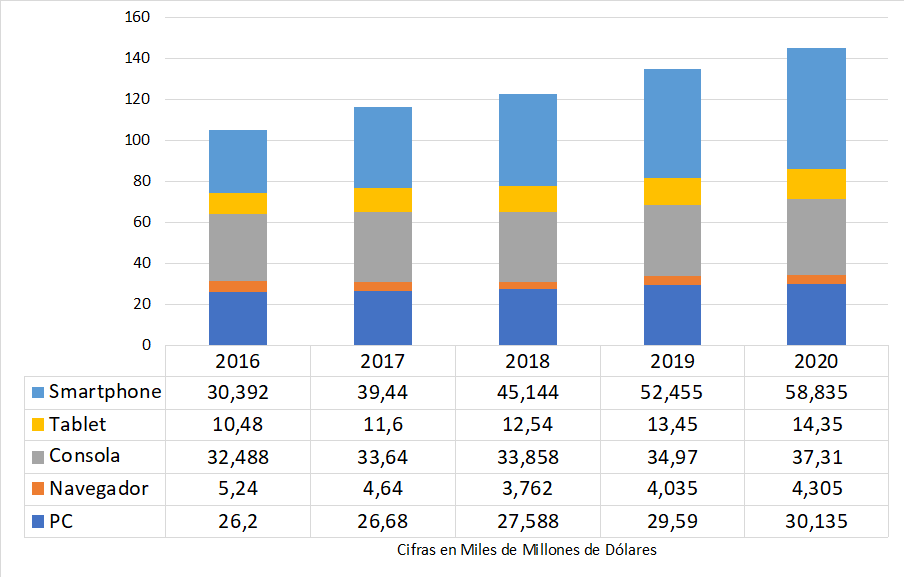
\includegraphics[width=0.8\textwidth]{images/estadodelarte/mercado/crecimiento_mercado_plataforma}
    \caption{Crecimiento mundial de la industria del videojuego (por plataformas).}
    \label{crecimiento_mercado_plataforma}
\end{figure}

Actualmente, la plataforma de distribución que ocupa un segmento mayor del mercado son los \textbf{dispositivos móviles}. Debido al constante incremento de potencia de los teléfonos inteligentes, así como a su ubicuidad en la sociedad actual, el mercado de videojuegos para estas plataformas ha experimentado un incremento constante en los últimos años, superando al mercado para PC y al mercado para videoconsolas de sobremesa. A fecha de 2017, el mercado de los juegos para teléfonos inteligentes ha alcanzado los \textbf{39.440 millones de dólares}, lo que representa el 34\% del mercado. Por otro lado, el mercado de las consolas portátiles y el de los juegos web casuales son los que presentan un declive más pronunciado, debido seguramente a que ocupan un nicho de mercado similar al de los juegos móviles \cite{libro_blanco}.

El mercado del videojuego se encuentra liderado por la región de \textbf{Asia Pacífico}, la cual incluye a países como China, Japón y Corea del Sur entre otros. Esta región por si sola supone prácticamente la mitad de los ingresos globales, con un total de 57.800 millones de dólares generados en el año 2017, de los cuales 32.5 millones fueron producidos solamente por China. Detrás del gigante asiático se encuentra \textbf{Estados Unidos}, que representa casi la totalidad de los ingresos de la región norteamericana con un total de 25.4 millones de dólares; y Japón, cuya producción asciende a los 14 millones. Por detrás de las principales potencias se encuentran varios países europeos: Alemania, Francia, España e Italia; sin embargo, como puede verse en la figura \ref{distribucion-mercado-mundial}, la diferencia en tamaño con respecto a los tres primeros mercados de la lista es abismal \cite{libro_blanco}.
\begin{figure}[!t]
    \centering
    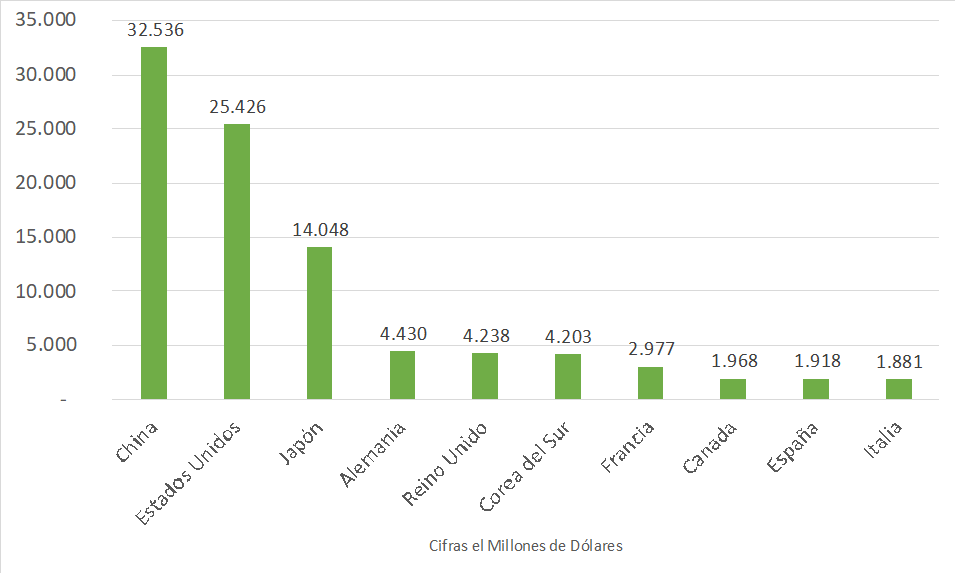
\includegraphics[width=1\textwidth]{images/estadodelarte/mercado/10-mayores-mercados}
    \caption{Distribución por países del mercado del videojuego.}
    \label{distribucion-mercado-mundial}
\end{figure}

\subsection{La industria de los videojuegos en España}
La industria del videojuego española es la \textbf{cuarta mayor de Europa} (como aparece en la figura \ref{distribucion-mercado-europa}) y la novena mayor a nivel mundial. A fecha de 2017, el mercado español del videojuego facturó un total de 1.900 millones de dólares, con un crecimiento del 20\% con respecto al año anterior. Más de la mitad de estos ingresos provienen de la \textbf{venta de videojuegos españoles al extranjero}, gracias a la casi total falta de fronteras para la distribución internacional de productos. Este enfoque en el mercado internacional se ve reflejado en factores como la mayor frecuencia del inglés en las producciones españolas que el propio español (99\% contra 95\%) \cite{libro_blanco}.
\begin{figure}[!t]
    \centering
    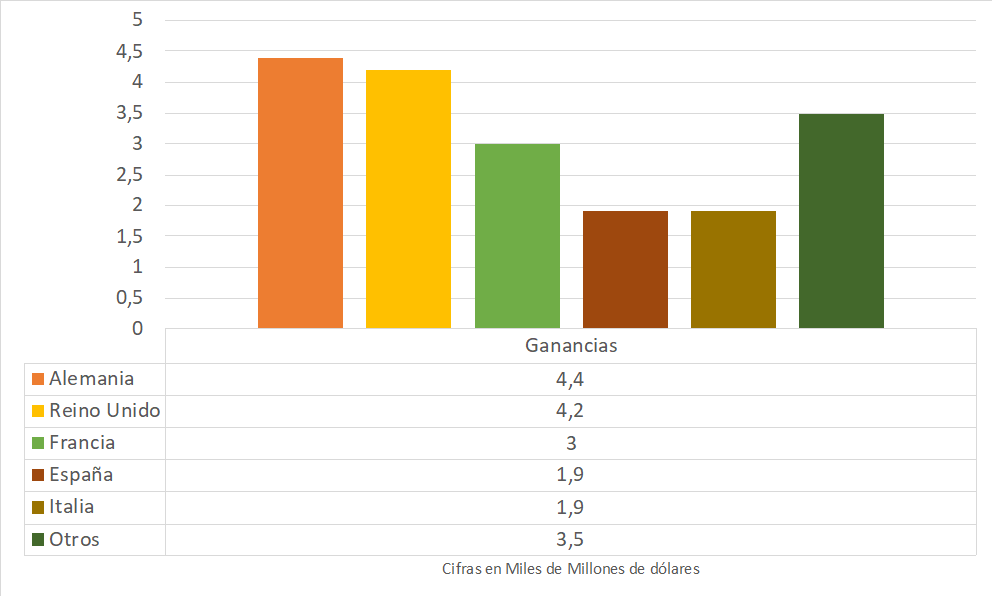
\includegraphics[width=0.8\textwidth]{images/estadodelarte/mercado/distribucion-mercado-europa}
    \caption{Mercado del videojuego en Europa.}
    \label{distribucion-mercado-europa}
\end{figure}

En total, el sector cuenta con \textbf{480 empresas en activo}, sin contar con las más de 100 iniciativas y proyectos empresariales, que se encuentran a la espera de consolidarse como empresas en el corto o medio plazo. En la figura \ref{distribucion-tamano-esp} se puede apreciar que la mayor parte de estas empresas tienen una plantilla de menos de 5 empleados, formando el 47\% de la industria. Esto se debe en parte a la adecuación de las pequeñas empresas a la creación de juegos de pequeña escala para dispositivos móviles (el principal mercado), pero también se debe a una escasez de puestos de trabajo en las empresas de tamaño mediano y grande y a la saturación del mercado que dificulta el crecimiento de las empresas \cite{libro_blanco}.
\begin{figure}[!t]
    \centering
    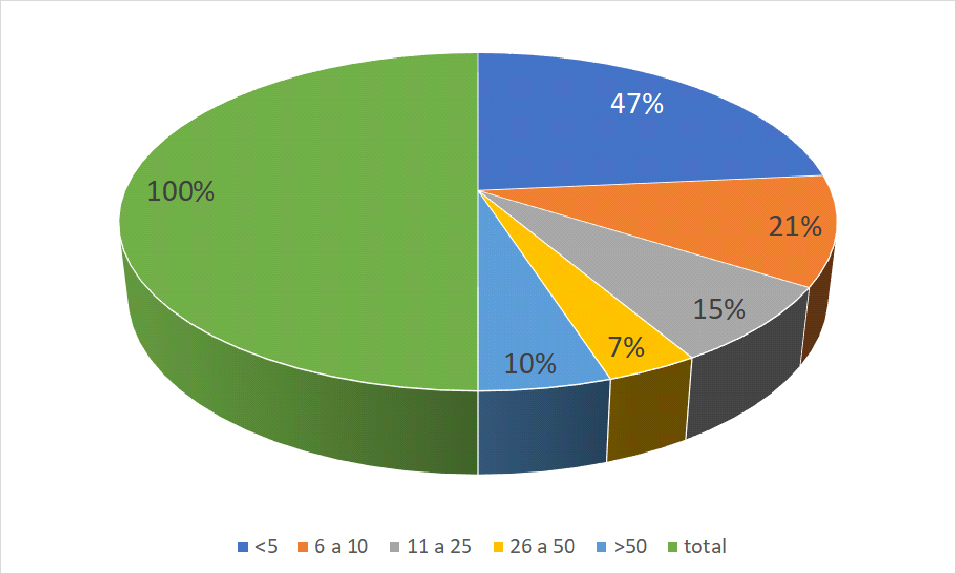
\includegraphics[width=0.8\textwidth]{images/estadodelarte/mercado/distribucion-tamano-esp}
    \caption{Distribución de las empresas en España por número de empleados.}
    \label{distribucion-tamano-esp}
\end{figure}

La actividad empresarial del país se encuentra centrada en dos comunidades autónomas: \textbf{Cataluña} y \textbf{la comunidad de Madrid}. De estos dos centros principales destaca Cataluña, donde se concentra el 52\% de la facturación del país. Detrás de las dos comunidades principales se encuentran la Comunidad Valenciana, el País Vasco y Andalucía, las cuales suman entre las tres un 28\% de las empresas. El resto de las comunidades se quedan muy por detrás de estas cinco primeras como puede verse en la figura \ref{distribucion-comunidades-esp} \cite{libro_blanco}.
\begin{figure}[h]
    \centering
    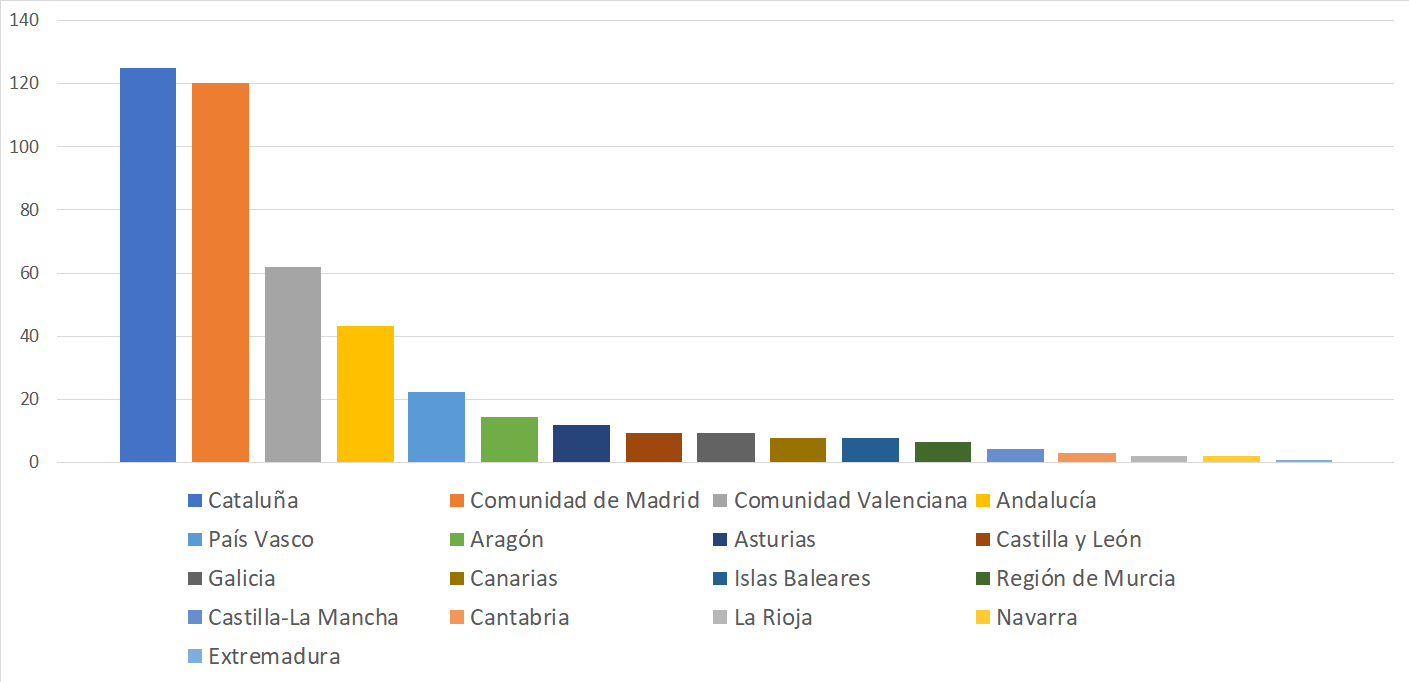
\includegraphics[width=0.8\textwidth]{images/estadodelarte/mercado/distribucion-comunidades-esp}
    \caption{Distribución de las empresas en España por número de empleados.}
    \label{distribucion-comunidades-esp}
\end{figure}

\subsection{Retos y tendencias actuales}
El videojuego ha sido y siendo una industria muy cambiante, que siempre ha intentado integrar las tecnologías más punteras, desde innovadores algoritmos de renderizado gráfico hasta exóticos dispositivos de interacción persona-ordenador. Las principales tendencias que van a influir fuertemente en el mercado en los años venideros son las siguientes:

\subsubsection{eSports}
Los eSports, también llamados \textbf{``deportes electrónicos''}, es el nombre por el cual se conocen las competiciones de videojuegos multijugador. En los eSports, los jugadores profesionales compiten entre ellos en juegos de diversos géneros: disparos en primera persona, lucha, estrategia en tiempo real, MOBAs (Multiplayer Online Battle Arena, ver figura \ref{foto-lol}) entre otras. La popularidad de este fenómeno ha llegado al punto en el que los grandes torneos como el \textbf{Intel Extreme Masters} (figura \ref{foto-torneo-esport}) se celebran en grandes estadios, están retransmitidos en streaming por Internet e incluso están dotados con premios de grandes sumas de dinero y que en ocasiones superan el millón de euros \cite{libro_blanco}.
\begin{figure}[!t]
    \centering
    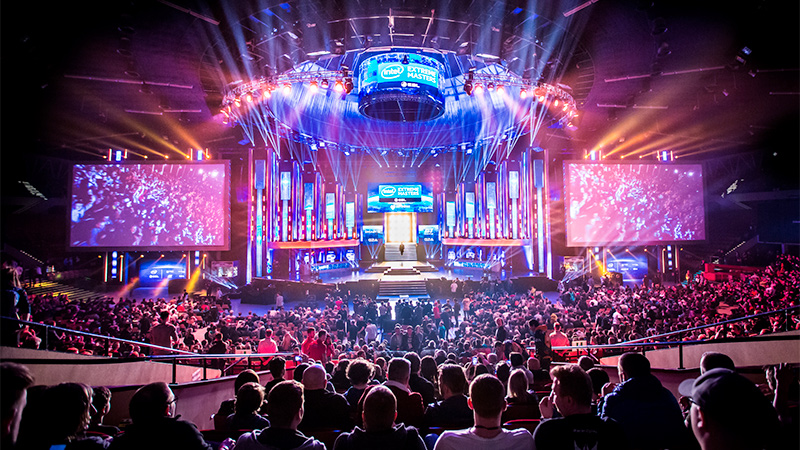
\includegraphics[width=0.8\textwidth]{images/estadodelarte/mercado/foto-torneo-esport}
    \caption{Fotografía del torneo Intel® Extreme Masters en Katowice, Polonia (Fuente: intelextrememasters.com)}
    \label{foto-torneo-esport}
\end{figure}

Actualmente, el impacto económico del mercado del eSport sigue siendo relativamente bajo, con unos ingresos de solo 660 millones de dólares en el año 2017. Esto se debe en parte a que \textbf{el gasto anual del ``aficionado'' medio es mucho menor que el de los aficionados a los deportes tradicionales} (3,64 dólares frente a 54) lo cual frena las inversiones de muchas compañías patrocinadoras. Sin embargo, las perspectivas de crecimiento son del 35,9\% anual, lo que provocará que para el año 2020 se alcance la cifra de los 1.504 millones de dólares, como se puede apreciar en la figura \ref{crecimiento-esport}.

\begin{figure}[!t]
    \centering
    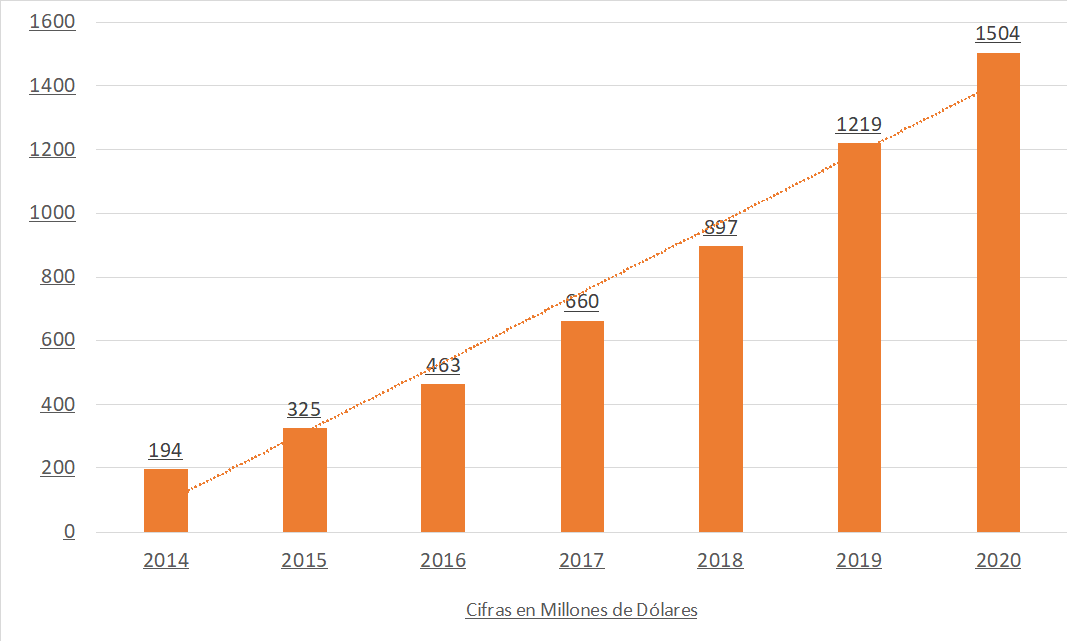
\includegraphics[width=1\textwidth]{images/estadodelarte/mercado/crecimiento-esport}
    \caption{Crecimiento del mercado del eSport (Fuente: \cite{libro_blanco}).}
    \label{crecimiento-esport}
\end{figure}

Otro factor que frena el crecimiento de los eSport es el enorme coste de su producción. En la mayoría de los casos, los eSports \textbf{surgen de manera orgánica} alrededor de juegos con una importante comunidad online de jugadores. Para reproducir estas condiciones, las empresas deben realizar importantes inversiones en infraestructura, personal dedicado a la comunidad, servidores escalables para una gran masa de jugadores o premios para los torneos. 

Sin embargo, esta inversión \textbf{no asegura que un producto tenga éxito} como eSport. Para que un videojuego pueda convertirse en un eSport necesita contar con características básicas: tener un fuerte factor de competición, partidas cortas de no más de 1 hora, sin progresión in-game (la progresión debe basarse en las habilidades del jugador) atractivo sistema de espectador y tener un enfoque al 100\% internacional.

Pese a su gran dificultad, conseguir posicionar un producto como eSports, aporta una serie de beneficios y posibilidades: 
\begin{itemize}
\item Crear una \textbf{base de fans}, una comunidad, algo que aporta un núcleo de consumidores fieles al producto y que le da una nueva dimensión social, muy atractiva para muchos de los consumidores de videojuegos.
\item \textbf{Prolongar la vida del producto}; al ser competitivo, el jugador fija sus metas ante los otros jugadores, esto incentiva al usuario y le proporciona una motivación para seguir consumiendo.
\item \textbf{Proporcionar mayor visibilidad}, ya que a pesar de que los productos asentados son extremadamente sólidos, su número es muy reducido, por lo cual hay una demanda latente de usuarios que buscan nuevos eSports.
\item \textbf{Aumentar la fidelidad de los usuarios} al tratarse de un mercado donde los usuarios tienen un índice de fidelidad mucho más alto que en otros.
\item Los jugadores, al estar involucrado con un producto competitivo, ven streaming, leen noticias, siguen torneos, participan en foros, lo que \textbf{disminuye el riesgo de abandono del producto}.
\end{itemize}
\begin{figure}[!t]
    \centering
    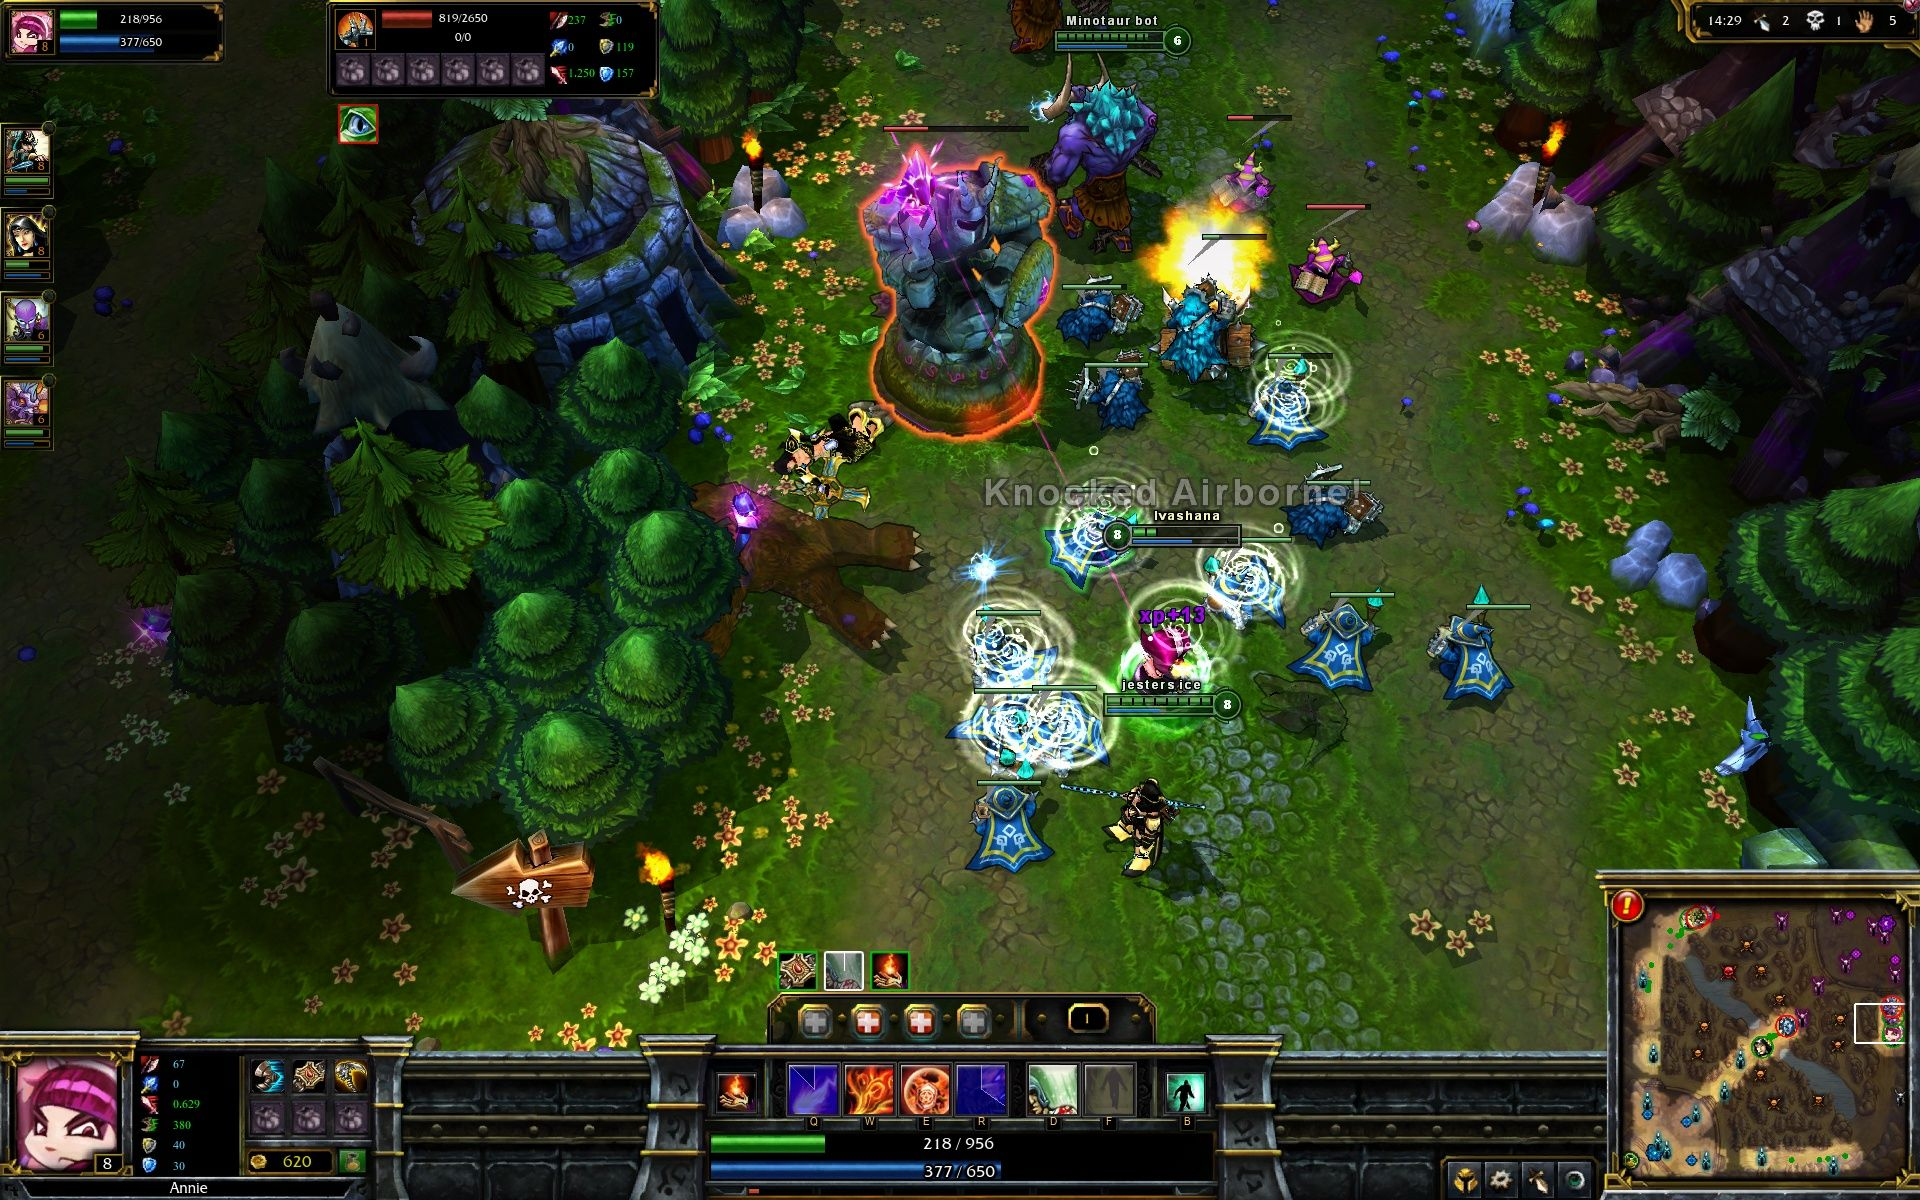
\includegraphics[width=0.8\textwidth]{images/estadodelarte/mercado/foto-lol}
    \caption{\citegame{league_of_legends}, uno de los eSports más populares (Fuente: mobygames.com).}
    \label{foto-lol}
\end{figure}

Para una empresa pequeña, la producción de un eSports es, en principio, inabarcable. Esto se debe principalmente la elevada inversión mencionada anteriormente. Sin embargo, en \textbf{asociación con grandes compañías} que puedan invertir en la infraestructura y publicidad necesaria, los pequeños estudios de desarrollo pueden tener una ventaja gracias a su flexibilidad para adaptarse a los cambios intrínsecos de un mercado nuevo. 

\subsubsection{Realidad Virtual y Realidad Aumentada}
La \textbf{Realidad Virtual} (normalmente abreviada como VR por las siglas inglesas de Virtual Reality) es la tecnología generada por sistemas informáticos que proporcionan un entorno audiovisual en 3D el que el usuario puede experimentar una inmersión total. Para ello, se hacen usos de cascos especiales equipados con pantallas y sensores de movimiento, los cuales se complementan con mandos equipados también con sensores para permitir una interacción más natural con el entorno virtual.

Por otro lado, la \textbf{Realidad Aumentada} o AR es una tecnología que superpone una capa de gráficos generados por ordenador sobre el entorno que rodea al jugador, con la que este puede interaccionar en tiempo real. A diferencia de la VR, no se requiere obligatoriamente de un hardware especial para poder implementar AR; basta únicamente de un dispositivo equipado con una pantalla y una cámara de vídeo, como podría ser un Smartphone.

El sector de la realidad virtual facturó en el año 2016 un total de \textbf{2.700 millones de dólares}, 1.100 millones menos de lo previsto según las estimaciones iniciales, mientras que la realidad aumentada generó un total de 1.200 millones de dólares, gracias en gran parte al éxito de \citegame{pokemon_go}. Pese a este lento inicio, las previsiones de crecimiento siguen siendo positivas, alcanzando los 108.000 millones de dólares en el año 2021, como se puede ver en la figura \ref{crecimiento-vr} \cite{libro_blanco}.
\begin{figure}[!t]
    \centering
    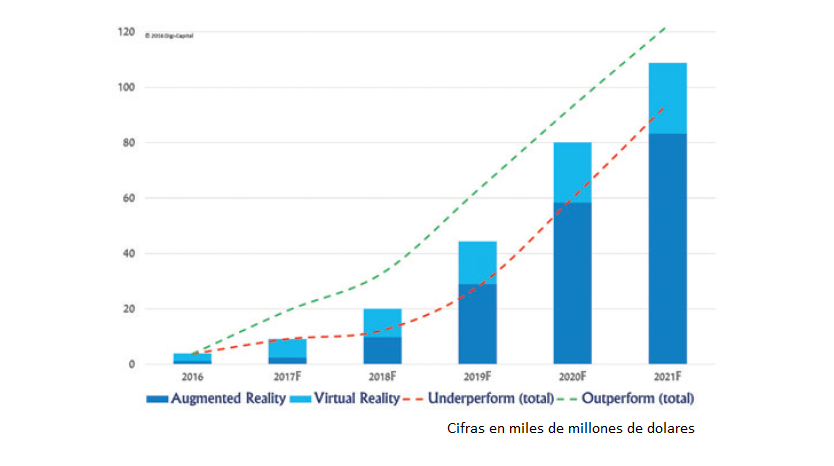
\includegraphics[width=1\textwidth]{images/estadodelarte/mercado/crecimiento-vr}
    \caption{Previsiones de crecimiento del mercado de Realidad Virtual y Aumentada (tabla extraída de \cite{libro_blanco}) (miles de millones de dólares).}
    \label{crecimiento-vr}
\end{figure}

Actualmente, existen varias propuestas de diversas compañías en lo que a equipo de VR se refiere. Estas son algunas de las propuestas más importantes:
\begin{itemize}
\item \textbf{HTC Vive\footnote{https://www.vive.com/}}: es la propuesta de HTC y Valve, orientada a jugadores ``hardcore'' de PC. Disponible desde abril de 2016, el dispositivo requiere de un PC de gama alta (Valve recomienda un PC con una gráfica GeForce GTX 970). El kit de hardware incluye el casco equipado con dos pantallas de 1080x1200 puntos y 90Hz de frecuencia de actualización, dos sensores espaciales y dos mandos para registrar los movimientos de ambas manos, lo que crea le permite crear un entorno 100\% virtual en el que sumergir al jugador.

\item \textbf{OCULUS Rift\footnote{https://www.oculus.com/rift/}}: Es la propuesta más veterana de la lista. Empezó como un exitoso proyecto de Kickstarter en 2012 que más tarde fue adquirida por la empresa Facebook dos años más tarde. Al igual que HTC Vive, Oculus está formado por un casco equipado con pantallas de alta resolución, mandos con sensores de movimiento y dos sensores de posición. El equipo necesita estar conectado a un PC de alta gama para poder funcionar correctamente.

\item \textbf{Samsung Gear VR\footnote{http://www.samsung.com/es/wearables/gear-vr-sm-r325nzvaphe/}}: La propuesta de Samsung es mucho más sencilla y económica, orientado más a la reproducción de vídeo en 360º (concepto similar a la realidad virtual, pero con interactividad limitada). El casco incluye una única pantalla y sus mandos carece de detección de movimiento. Estas limitaciones conllevan, por otro lado, un precio mucho más accesible que el de las otras alternativas (99€ contra los más de 500€ de las propuestas más completas)

\item \textbf{SONY PlayStation VR\footnote{https://www.playstation.com/explore/playstation-vr/}}: la propuesta de Sony fue lanzada en el año 2016. Al igual que otras alternativas, el sistema se basa en un casco equipado con dos pantallas y sensores de movimiento, pero su principal punto de venta es su compatibilidad con la consola PlayStation 4 de la misma marca. Esto permite aprovechar la potencia y los mandos de control de está de la consola.
\end{itemize}
En la figura \ref{fotos_vr} se puede ver una fotografía de cada uno de los dispositivos descritos.
\begin{figure}[!htb]
   \begin{minipage}{0.24\textwidth}
     \centering
     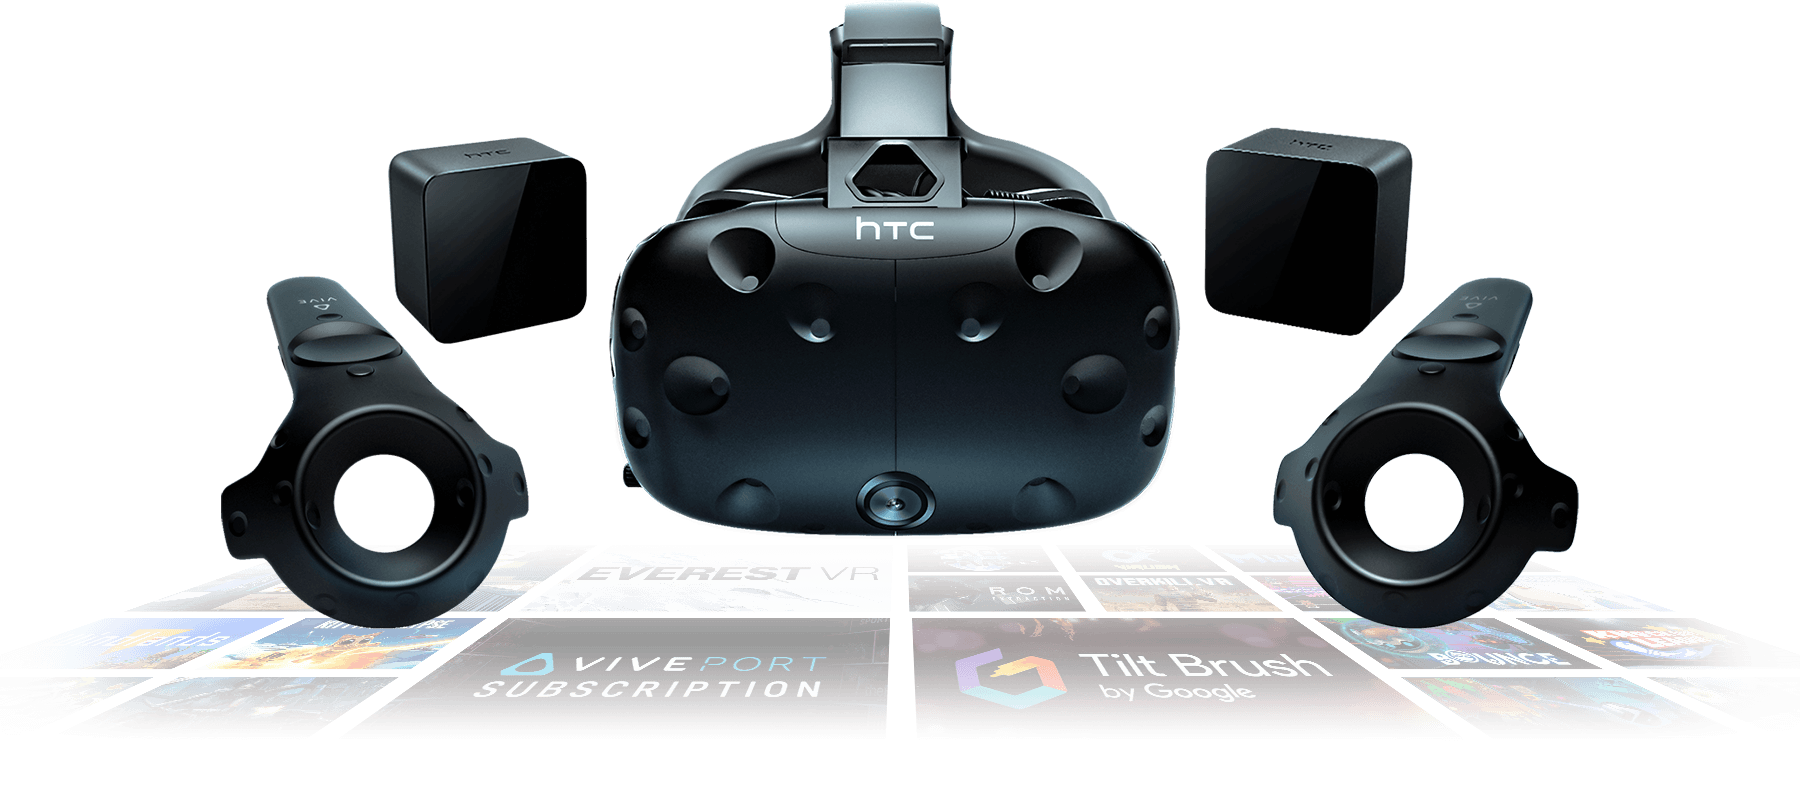
\includegraphics[width=0.7\linewidth, right]{images/estadodelarte/mercado/foto-htc-hive}
   \end{minipage}\hfill
   \begin {minipage}{0.24\textwidth}
     \centering
     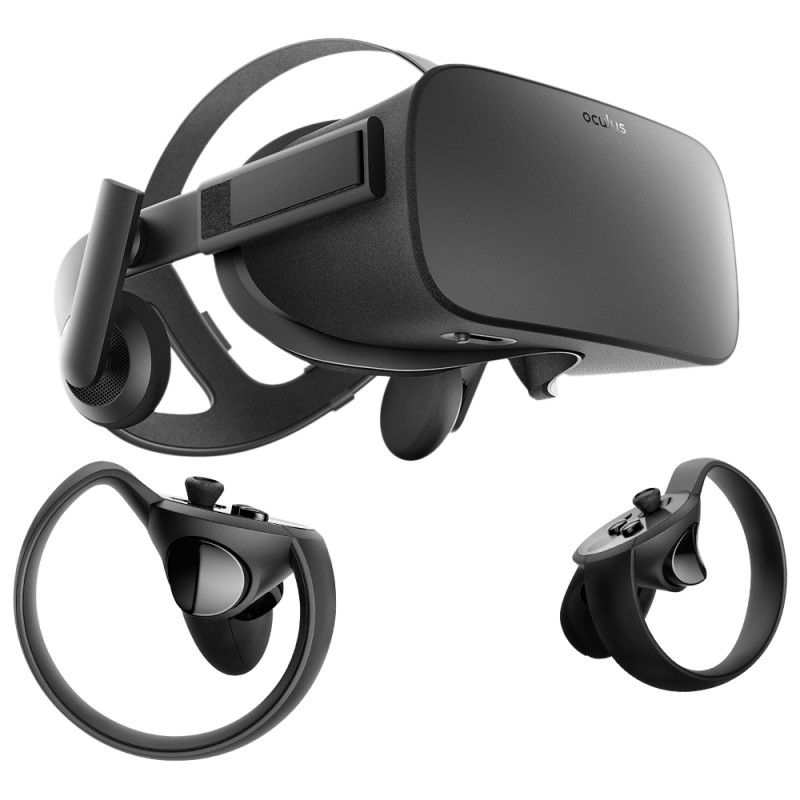
\includegraphics[width=0.7\linewidth, left]{images/estadodelarte/mercado/foto-oculus}
   \end{minipage}
      \begin {minipage}{0.24\textwidth}
     \centering
     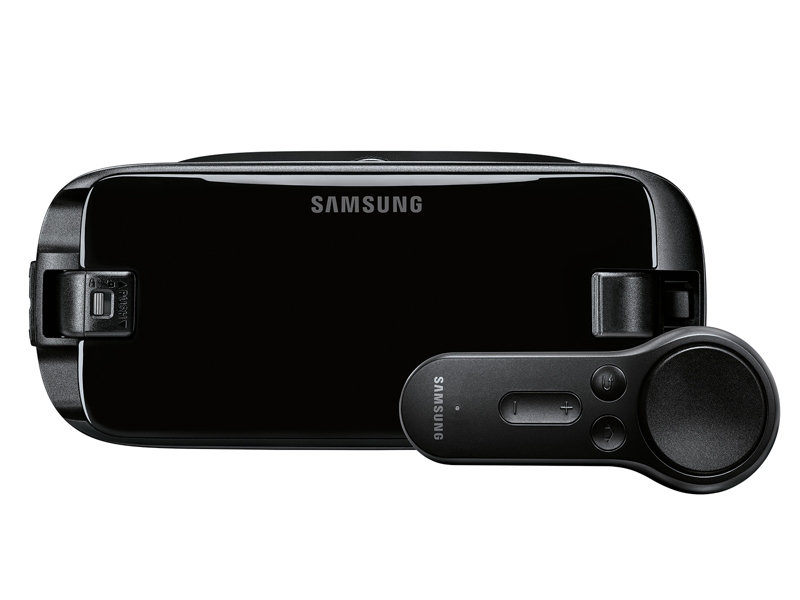
\includegraphics[width=0.7\linewidth, left]{images/estadodelarte/mercado/foto-samsung-vr}
   \end{minipage}
      \begin {minipage}{0.24\textwidth}
     \centering
     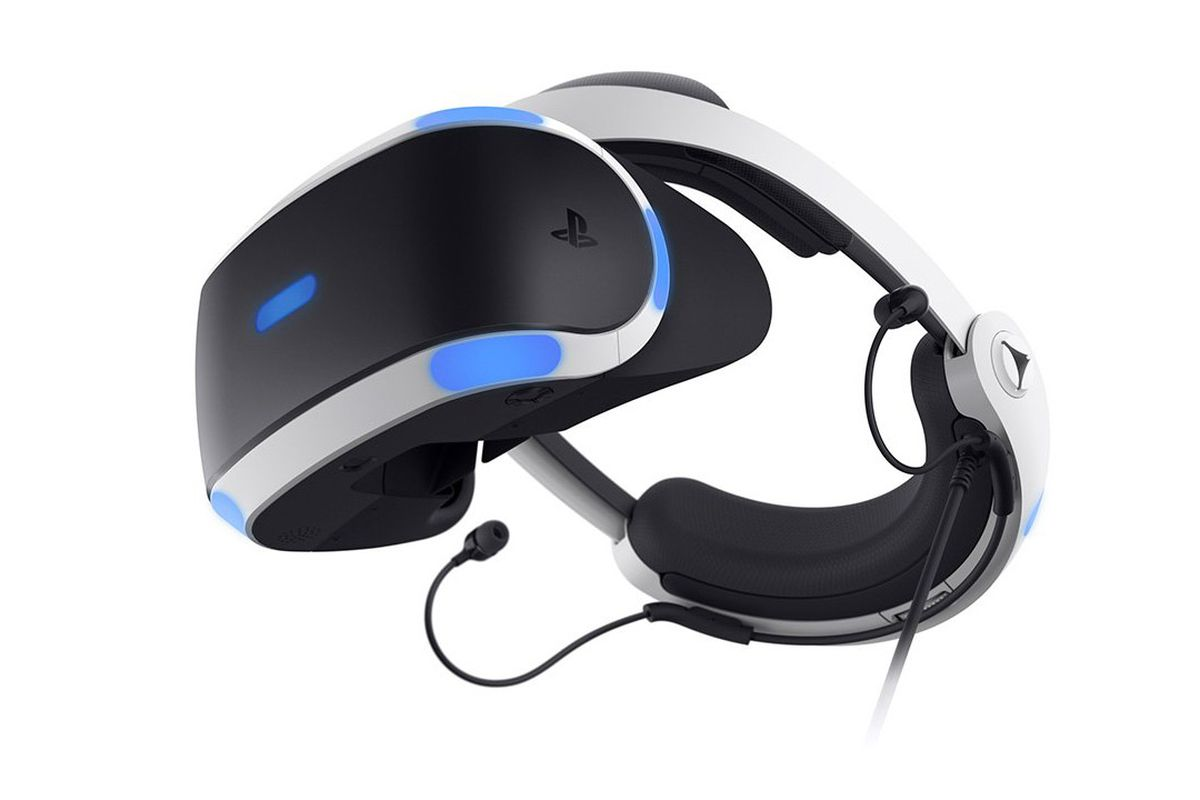
\includegraphics[width=0.7\linewidth, left]{images/estadodelarte/mercado/foto-sony-vr}
   \end{minipage}
   \caption{De izquierda a derecha: HTC Vive, Oculus Rift, Samsung VR y PlayStation VR (imágenes tomadas de las páginas oficiales de los productos).}
	\label{fotos_vr}
\end{figure}

\subsubsection{Web 4.0}
El termino Industria 4.0 fue acuñado por el \textbf{Ministerio de Educación y Desarrollo alemán} en su plan estratégico de 10 puntos del año 2016 para mejorar la educación, investigación e industria del país para adaptarlas a las tecnologías de Internet \cite{web_4_0}. La estrategia trata cinco áreas principales:
\begin{itemize}
\item Fuerte cooperación entre la investigación científica y las empresas.
\item Aumentar la innovación en el sector privado.
\item Diseminar las tecnologías punteras.
\item Internacionalizar la investigación y desarrollo.
\item Fondos para individuos con talento.
\end{itemize}

De entre las distintas tecnologías que podrían categorizarse como parte de la industria 4.0, Las que tienen una aplicación más directa en el desarrollo de videojuegos son las siguientes \cite{libro_blanco}:

La computación en la nube, o \textbf{Cloud Computing}, es la tecnología que permite el acceso a servicios informáticos de forma rápida y sencilla a través de Internet. Aunque aún no se ha podido implementar correctamente el \textbf{Cloud Gaming} (donde el juego es íntegramente ejecutado en la nueve, reduciendo la exigencia de potencia del sistema del jugador), si se utilizan sistemas en la nube en distintas áreas de los videojuegos. Especialmente notable es su uso para el control y almacenamiento de información en juegos multijugador en línea.

\textbf{El Internet de las cosas} es como se conoce a la tecnología que permite dotar de conexión a Internet a todo tipo de pequeños dispositivos como relojes, sistemas de domótica, drones, sensores de todo tipo, robots, etc. Esto permite implementar videojuegos en todo tipo de sistemas, desde consolas portátiles cada vez más pequeñas y económicas, pasando por juguetes interactivos y llegando a la posibilidad de gamificar con facilidad procesos industriales.

\textbf{Big Data} es el proceso de clasificar grandes volúmenes de datos para poder obtener relaciones interesantes y no evidentes entre ellos. El principal uso de las técnicas de BigData en la industria del videojuego es el análisis de la información de los jugadores. Analizando datos de los jugadores tales como el género, la edad, la localización geográfica, los intereses, los gastos realizados, etc. es posible obtener estrategias de negocios eficientes.

\textbf{Los sistemas Ciberfísicos} son un nuevo tipo de sistemas con unos componentes hardware y software estrechamente interconectados, cada uno operando en su propio ámbito, operando e interaccionando de forma distinta dependiendo del contexto \cite{cyber_physics}. Entre sus aplicaciones se encuentran las redes eléctricas inteligentes, los sistemas de conducción automática de aviones y automóviles o la monitorización médica. Para la correcta manipulación de estos sistemas se requieren de unas interfaces de usuario con un fuerte ``lado humano'' que permita un uso sencillo e intuitivo. Aquí se podrían utilizar los principios de diseño de juego que permitirían desarrollar un mejor puente entre el lado máquina y la parte de usuario.

\textbf{La Impresión 3D}, también conocida como la producción aditiva es una tecnología que permite producir objetos de forma más sencilla que con las técnicas anteriores gracias a máquinas como la mostrada en la figura \ref{impresion-3d}. En combinación con las técnicas de escaneado 3D, los estudios de videojuego pueden generar de forma rápida y eficiente modelos 3D de todo tipo (personajes, mapas, objetos...).

\begin{figure}[h]
    \centering
    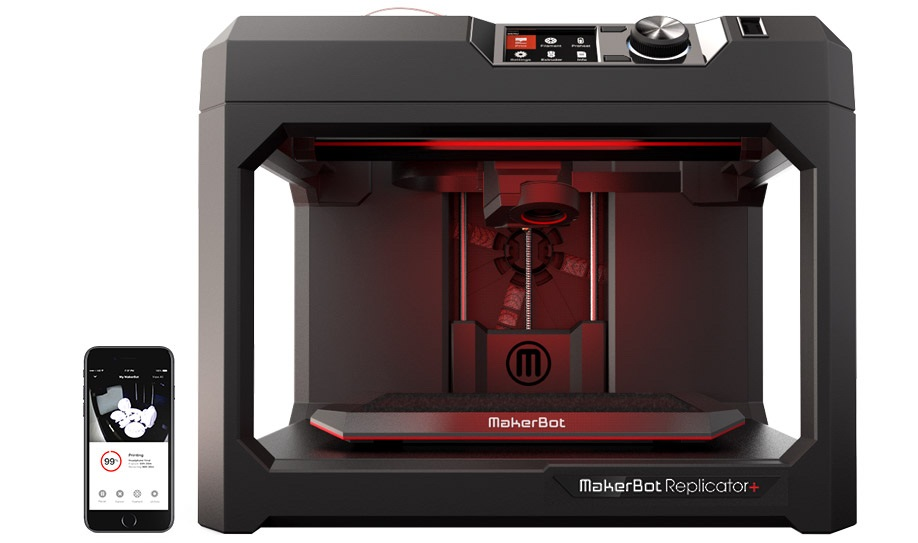
\includegraphics[width=0.8\textwidth]{images/estadodelarte/mercado/impresion-3d}
    \caption{Impresora 3d ``replicator'' de la compañía Makerbot.}
    \label{impresion-3d}
\end{figure}

Las nuevas tecnologías de la industria 4.0 serán de gran ayuda para el desarrollo de videojuego. Pero es posible que la industria 4.0 también ofrezca valor a la industria 4.0 en su conjunto. Dado que la creación de videojuegos es una actividad industrial que está vinculada a diferentes áreas de conocimiento que trabajan juntas para conseguir ofrecer un producto, las técnicas y \textbf{paradigmas utilizados tienen mucho en común con la nueva forma de trabajar de la industria 4.0}, por lo que es posible que puedan extrapolarse a otras industrias, permitiendo una mejor adaptación a los cambios.

\section{El proceso de desarrollo de videojuegos}
El desarrollo de un videojuego, como el de cualquier otro producto software, debe de ser planificado correctamente y ejecutado siguiendo una metodología adecuada. Sin embargo, el diseño y desarrollo de un videojuego requiere de la participación de campos ajenos a la informática como el diseño de juegos, el diseño gráfico o la composición musical. Una parte importante de la producción consistirá en organizar a un equipo multidisciplinario para poder terminar el proyecto dentro del tiempo y presupuesto acordados \cite{libro_esi}.

\subsection{Etapas del desarrollo}
El proceso de desarrollo de videojuegos difiere del de otros tipos de software, debido a la necesidad de integrar en un mismo producto elementos de diferentes disciplinas. En ese sentido, el desarrollo de un videojuego \textbf{es similar a la producción de una película de cine}, para las cuales también es necesario coordinar el trabajo de profesionales de áreas muy diversas. Partiendo en esta similitud, el desarrollo de videojuego suele organizarse en las tres etapas en las que se divide la producción de una película: \textbf{pre-producción}, \textbf{producción} y \textbf{postproducción}.

Para organizar el trabajo en cada una de estas etapas, se suele utilizar el \textbf{modelo en cascada de Royce}, el cual se basa en realizar las tareas de forma lineal \cite{libro_esi}. En la figura \ref{etapas-desarrollo} y en los siguientes apartados se describe el desarrollo basándose en este modelo. 
\begin{figure}[!t]
    \centering
    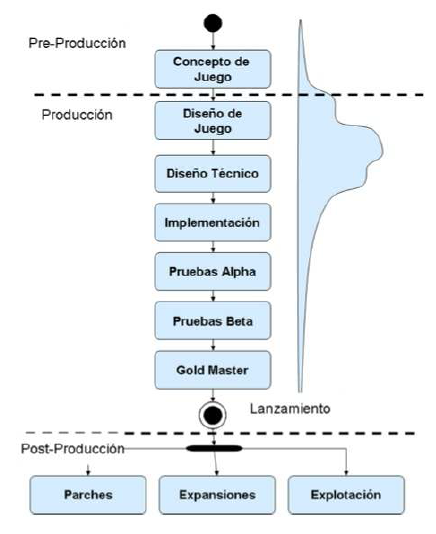
\includegraphics[width=0.65\textwidth]{images/estadodelarte/desarrollo/etapas-desarrollo}
    \caption{Etapas del desarrollo de un videojuego (Imagen tomada del \cite{libro_esi}.}
    \label{etapas-desarrollo}
\end{figure}

\subsubsection{Desarrollo del Concepto}
El desarrollo de todo videojuego comienza con una idea. Durante la fase de desarrollo del concepto se tomará dicha idea para obtener un \textbf{diseño preliminar} listo para preproducción. El objetivo principal de esta etapa es decidir sobre qué tratará el juego y ponerlo por escrito para que cualquier miembro del equipo lo pueda entender con claridad, decidiendo las principales mecánicas, creando el arte conceptual y escribiendo el argumento\cite{game_design_2}. 

Al final de la etapa se habrán elaborado tres documentos: El \textbf{\textit{high concept}}, el \textbf{\textit{pitch document}} y el \textbf{\textit{concept document}}. El \textbf{\textit{high concept}} consiste en una o dos frases que describen a grandes rasgos cómo será el juego, en especial que lo hace distinto de la competencia. El \textbf{\textit{pitch document}}, o ``propuesta de juego'', es un pequeño documento de en torno a dos páginas, orientado a ser leído en las reuniones donde el juego sea propuesto a inversores. El documento resume las características del juego y explica por qué será exitoso y rentable.

Finalmente, \textbf{\textit{concept document}} es un extenso documento que explica en detalle las características del juego. Se trata de una versión extendida de \textit{pitch document} que trata temas como: 
\begin{itemize}
\item El high concept
\item El género del juego
\item Características principales y jugabilidad.
\item Ambientación e historia.
\item Estimación del presupuesto y de la planificación.
\item Equipo de desarrollo.
\item Análisis de riesgos.
\end{itemize}

\subsubsection{Pre-Producción}
La preproducción es la fase de preparación: en la que el equipo diseña y planifica los elementos que serán desarrollados en la etapa de producción. Al final de esta etapa, se debe haber completado el \textbf{diseño de juego}, creado la \textbf{biblia de arte}, elaborado el \textbf{documento de diseño técnico}, establecido el \textbf{plan de producción}, y creado un \textbf{prototipo del juego final} \cite{game_design_2}.

El diseño del juego quedará establecido en un \textbf{documento de diseño de juego} (o GDD, por sus siglas en ingles). Se trata de un documento ``vivo'', que está en constante modificación para adaptarse a los ajustes concretos de diseño que se realizarán durante el desarrollo.

\textbf{La biblia de arte} es una colección de arte conceptual que servirá para definir el estilo artístico del juego desde un primer momento. La biblia incluirá también una librería de imágenes de referencia que puedan ser de ayuda a los artistas que desarrollen los elementos gráficos finales.

\textbf{El documento de diseño técnico} contiene una descripción en detalle la parte técnica del proyecto definiendo las tareas que los desarrolladores deberán afrontar, estimando el coste que dichas tareas tendrán tanto en tiempo como en número de personas y especificando las herramientas y técnicas que utilizará el equipo.

\textbf{El Plan de Producción} recopila la información acerca de cómo se va a desarrollar el proyecto. Este incluye las tareas a realizar junto a los tiempos, costes y dependencias de estas, divididos en varios documentos menores para poder ser organizado mejor:
\begin{itemize}
\item \textbf{Plan de mano de obra}: Listado del personal, sus horarios y su salario.
\item \textbf{Plan de recursos} Estimación del coste los recursos externos al proyecto (música, arte, herramientas...)
\item \textbf{Documento de seguimiento}: Documento donde se realiza un control de los tiempos y plazos del proyecto.
\item \textbf{Presupuesto}: Contiene el coste mensual del proyecto y el cálculo del presupuesto general
\item \textbf{Ganancias y pérdidas}: Estimación  de las ganancias y  pérdidas del proyecto. Debe ir actualizándose según se avanza en el desarrollo.
\item \textbf{Definición de hitos}: Lista de las distintas ``metas'' del proyecto, que son puntos del desarrollo donde se habrá terminado una cantidad de trabajo importante.
\end{itemize}

Una vez diseñado y planificado el proyecto, el equipo empezara a trabajar en la creación de un \textbf{prototipo}. Un prototipo es una pieza de software funcional que contiene una pequeña fracción del software final. El desarrollo prototipo servirá para varias funciones: poner a prueba el diseño de juego, concretando de forma más precisa la jugabilidad; realizar un simulacro de desarrollo para determinar las dinámicas del equipo y producir una muestra del juego final a inversores y publicadores \cite{game_design_2}. 

\subsubsection{Producción}
\textbf{La producción} es la etapa principal del desarrollo del juego. Durante esta etapa se elaborarán e implementarán los elementos descritos y diseñados durante la preproducción: los programadores implementarán los sistemas del juego, los artistas elaborarán los gráficos definitivos, los diseñadores crearán misiones y niveles, etcétera. Dependiendo del juego en cuestión, una producción normal suele durar entre seis meses y dos años, aunque el desarrollo de juegos pequeños para, por ejemplo, dispositivos móviles puede realizarse en menos tiempo aún \cite{development_and_production}.

La etapa de producción es de \textbf{naturaleza iterativa}: El juego va construyéndose en varias etapas en las que se implementan pequeñas porciones de este. Entre etapa y etapa, el juego pasa por un proceso de pruebas en la que se verifica su usabilidad y robustez frente a fallos. Los resultados de las etapas se utilizan como base para recalcular los tiempos y presupuestos de las etapas posteriores. Dividir el desarrollo de esta forma hace que sea más sencillo afrontar problemas y contratiempos que el equipo podría encontrar en las etapas tardías.

\subsubsection{Final de Producción y Lanzamiento}
Durante las últimas etapas de la producción, el paradigma de desarrollo cambia, pasando el objetivo de implementar contenido nuevo a pulir y ajustar el contenido preexistente. Esta parte de la producción puede dividirse en dos etapas: Alpha y Beta.

La fase \textbf{Alpha} o Code-Complete es el punto del desarrollo donde el juego se encuentra en un estado jugable, a falta solo de ciertos vacíos como gráficos provisionales o minijuegos o subsistemas incompletos. El objetivo de esta etapa es el de encontrar y corregir todos los fallos posibles y también probar y ajustar la jugabilidad \cite{development_and_production}.

En la fase \textbf{Beta} o Content-Complete la mayor parte del contenido del juego deberá estar terminado y debe haber pocos o ningún fallo importante en el juego. En esta etapa el juego es puesto en manos de equipos de testing externos a la empresa para realizar análisis exhaustivos en busca de fallos que se le pueden haber escapado al equipo de testing interno. Es también en esta etapa donde la campaña de publicidad del juego deberá ser más fuerte \cite{development_and_production}.

Una vez superadas las dos etapas de pruebas, la \textbf{versión final} del juego es enviada a la distribuidora para que comience la producción de las copias físicas, o para que el juego aparezca en las plataformas de distribución.

\subsubsection{Postproducción}
Una vez lanzado el juego, el equipo entra en la etapa de \textbf{postproducción}. En esta etapa el equipo trabajará en corregir fallos y problemas que los jugadores encontraron tras el lanzamiento y en la elaboración de contenido adicional descargable.

La duración y trabajo de la posproducción depende mucho del juego en cuestión. Hasta hace relativamente poco, los juegos lanzados en videoconsolas carecían completamente de esta etapa debido a la dificultad para modificar los juegos que ya se encontrasen en el mercado. por otro lado, hoy en día la mayor parte de los videojuegos reciben parches y actualizaciones sin importar su plataforma de distribución \cite{development_and_production}.

Un caso especial sería el de los juegos con un fuerte componente online, como los \textbf{MMORPG}, los \textbf{MOBA} o los \textbf{shooter en línea}. Los desarrolladores de este tipo de juegos, para mantener contenta a su base de jugadores y evitar el estancamiento, lanzan de forma periódica actualizaciones que ofrecen nuevo contenido, mejoras y ajustes. Algunos de estos juegos pueden recibir este tipo de actualizaciones durante años, como \citegame{world_of_warcraft} o \citegame{team_fortress_2}, ambos en activo desde hace más de 10 años.

\subsection{Estructura típica de un equipo de desarrollo}
El desarrollo de un videojuego puede llevarse a cabo por equipos de desarrollo muy distinto dependiendo de la \textbf{extensión del proyecto}, desde una sola persona creando un pequeño juego independiente, el cual realiza todo el trabajo por sí mismo; hasta los equipos de cientos de personas que desarrollan los juegos AAA, organizados en múltiples departamentos, cada uno con su estructura jerárquica.

A pesar de esto, existen una serie de roles que están presentes en todos los desarrollos. En la figura \ref{table-roles} se puede ver la estructura de roles. Hay que tener en cuenta que una estructura tan completa solo aparece en los \textbf{grandes equipos}. En proyectos pequeños es normal persona ejerza varios roles, o incluso que una única persona lleve el desarrollo completo.
\begin{figure}[!t]
    \centering
    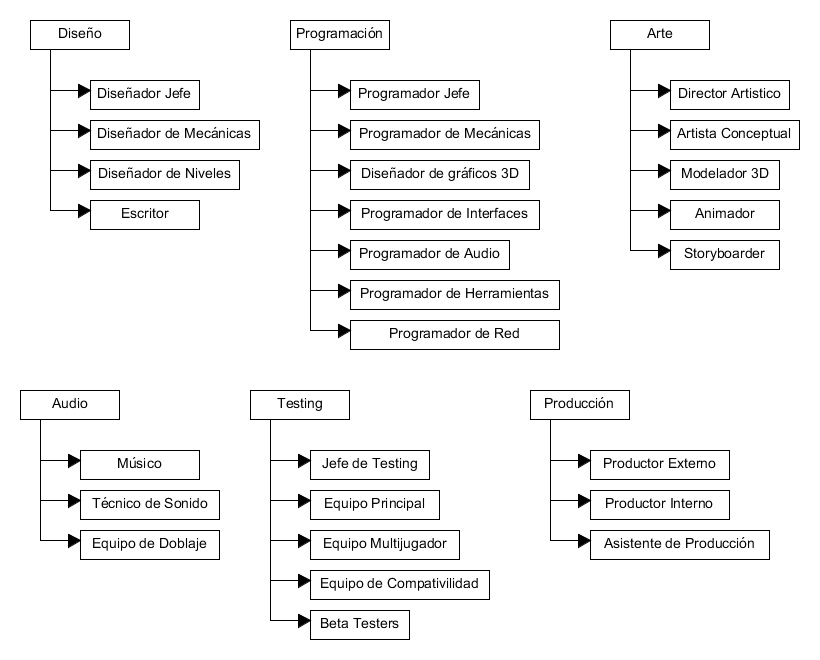
\includegraphics[width=1\textwidth]{images/estadodelarte/desarrollo/table-roles}
    \caption{Distribución de roles en un equipo de desarrollo.}
    \label{table-roles}
\end{figure}

\subsubsection{Diseño}
La primera y más importante parte del desarrollo de un juego es el \textbf{Diseño} de este. El trabajo del \textbf{diseñador} es de describir el juego con un alto nivel de detalle, definiendo de con precisión todas las mecánicas, personajes, mapas, misiones del juego. Deberá también, hasta cierto punto, coordinar y dirigir el trabajo del resto de miembros del equipo para que puedan implementar correctamente el juego. 

En equipos grandes, el rol de diseñador puede dividirse en las siguientes categorías \cite{development_and_production}:
\begin{enumerate}
\item \textbf{Diseñador jefe}: Es el encargado de dirigir al resto de diseñadores, decidiendo que contenido entra o no en el juego. Suele ser la persona que tuvo la ``idea'' original del juego.
\item \textbf{Diseñador de mecánicas}: El diseñador de mecánicas es el encargado de diseñar los distintos sistemas de juego, sirviendo como puente entre el diseñador jefe y los programadores. Debido a esto, el diseñador de mecánicas suele tener un trasfondo de programador.
\item \textbf{Diseñador de niveles}: También llamados diseñadores de misiones son los encargados de crear las distintas etapas que componen el juego, ya sean niveles, misiones, desafíos o puzles.
\item \textbf{Escritor}: La tarea del escritor es la de crear la historia del juego, así como la de escribir los distintos textos de este, como diálogos o descripciones. Se trata de una tarea muy distinta de la de un escritor de novelas o de guiones de película, ya que debe conciliar la narrativa con las exigencias de otros componentes del juego como el diseño, el arte o las limitaciones técnicas.
\end{enumerate}

\subsubsection{Programación}
El rol del \textbf{programador} es el de implementar el juego en forma de código ejecutable. Esto supone el diseño e implementación de todo tipo de componentes imprescindibles: motor de renderizado, librerías para trabajar con sistemas de audio o conectarse por Internet, herramientas para integrar fácilmente el contenido artístico entre otras.

Cuando el equipo de desarrollo es grande, el rol de programador tiende a dividirse para cubrir tareas más específicas \cite{development_and_production}:
\begin{enumerate}
\item \textbf{Programador jefe}: El programador jefe es frecuentemente el programador con más experiencia del equipo y él es el encargado de resolver las tareas más complicadas e importantes del proyecto. Cuando el equipo es muy grande, suelen realizar también tareas de coordinación.
\item \textbf{Programador de mecánicas}: Es el encargado de convertir el diseño de juego en código ejecutable. Entre sus tareas se encuentra definir las físicas del mundo del juego, definir las funciones de los distintos objetos y modelar el comportamiento de los personajes.
\item \textbf{Programador de gráficos 3D}: Es el responsable de implementar los sistemas para la creación y renderizado de gráficos 3D. El programador de gráficos 3D necesita contar con conocimientos avanzados en calculo, matemática vectorial y matricial, trigonometría y álgebra.
\item \textbf{Programador de interfaces}: Es el encargado de implementar los sistemas de interacción entre el jugador y el juego, normalmente interfaces de control, menús y HUDs (Head-Up Displays). 
\item \textbf{Programador de audio}: Es la persona responsable de la implementación de los distintos sistemas que se utilizarán para reproducir música y sonido en el juego
\item \textbf{Programador de herramientas}: El programador de herramientas tiene la responsabilidad de crear las distintas herramientas que el resto del equipo pueda necesitar para realizar, o acelerar, su trabajo. Un tipo especializado de programador de herramientas es el programador del editor de niveles, debido a la importancia de esta herramienta para el desarrollo del juego y por la posibilidad de que dicho editor sea lanzado al público como parte del juego.
\item \textbf{Programador de red}: Es el encargado de escribir el código que permite a los juegos ser ejecutados entre varios equipos, ya sea código máquina de bajo nivel o la integración de una librería de alto nivel.
\end{enumerate}

\subsubsection{Arte}
Se denomina \textbf{artista} a la persona o grupo encargado de generar los componentes gráficos del juego: modelos 3D de personajes y objetos, texturas, diseño de menús e interfaces, bocetos, animaciones y demás.

Existen varias categorías de artistas distintas dependiendo de en qué rama se especialicen y de cuál sea su rol en la estructura del proyecto \cite{development_and_production}:
\begin{itemize}
\item \textbf{Director artístico}: Asignado al artista con mayor experiencia en la industria, el papel del director artístico es el de organizar y coordinar al resto de artistas para que realicen correctamente su trabajo y el de revisar las piezas producidas para asegurarse de que son consistentes con el estilo artístico establecido.
\item \textbf{Artista conceptual}: El artista conceptual es el encargado de producir bocetos provisionales que servirán como base para construir los gráficos definitivos del juego.
\item \textbf{Artista 2D}: Los artistas 2D son expertos en las técnicas tradicionales del dibujo y pintura.  Su rol es más notable en los juegos 2D, donde deben producir la mayoría de los componentes gráficos como fondos, \textit{tiles} y \textit{sprites}; pero también tienen un papel notable en los juegos 3D, donde suelen ser los encargados de diseñar interfaces gráficas, crear las texturas de los modelos 3D e incluso realizar trabajos ajenos al propio juego como la creación de imágenes promocionarles.
\item \textbf{Modelador 3D}: Es el encargado de producir los modelos 3D de los distintos componentes del juego tales como personajes, objetos, mapas...  Es relativamente común que los modeladores 3D tengan ciertos conocimientos de programación debido a que eran necesarios para trabajar con los primeros programas de modelado 3d.
\item \textbf{Animador}: Es el encargado de animar los diferentes elementos del juego, desde el simple movimiento de un molino de viento hasta las complicadas expresiones de una cara. Existen dos alternativas para realizar la animación: la técnica de keyframing, que consiste en realizar poses estáticas de los personajes que el programa utiliza para generar la animación; y la captura de movimiento, en la que los movimientos de un actor son capturados y transferidos al juego mediante un equipo especializado.
\item \textbf{Storyboarder}: Es el artista encargado de diseñar escenas del juego. Para ello, el Storyboarder crea unas secuencias de arte conceptual que describen los tiempos, diálogos y eventos de las escenas, lo que permite valorarla y validarla antes de iniciar el costoso proceso de producción.
\end{itemize}

\subsubsection{Audio}
El trabajo de \textbf{audio} en un videojuego viene en tres categorías: música, efectos de sonido y doblaje. Existen especialistas que se dedican exclusivamente a una sola de estas categorías, aunque no es raro encontrarse en pequeños estudios a una persona encargarse tanto de la música como del sonido. Reflejando los tipos de audio, los tres tipos de profesionales son \cite{development_and_production}:
\begin{enumerate}
\item \textbf{Músico}: Es el artista encargado de escribir las composiciones musicales que se escucharán a lo largo del juego. Es muy común que el músico también se haga cargo de interpretar sus composiciones mediante programas de síntesis de música, aunque las grandes producciones pueden permitirse contratar interpretaciones en vivo.
\item \textbf{Técnico de sonido}: Los técnicos de sonido son profesionales que se dedican a fabricar o adaptar sonidos para el proyecto en el que trabajen.
\item \textbf{Equipo de doblaje}: El trabajo de doblar un videojuego requiere del trabajo de varios profesionales. En primer lugar, está el actor de voz, un actor especializado que interpreta con su voz a uno o varios personajes del juego. El trabajo de los actores está supervisado por un director de doblaje, que además suele encargarse de adaptar el guion y de dirigir a los técnicos de sonido que van a grabar y manipular las voces.
\end{enumerate}

\subsubsection{Testing}
\textbf{El aseguramiento de la calidad} (o QA por sus siglas en inglés) es un requisito clave para el desarrollo de un videojuego, a la vez de un proceso lento y costoso que debe comenzarse lo más pronto posible para evitar un sobrecoste \cite{development_and_production}. El trabajo del tester es el de revisar las distintas versiones del juego en busca de fallos para que los desarrolladores puedan arreglarlos.

Normalmente, los testers de un juego se agrupan en equipos, dirigidos por un \textbf{jefe de testing}. Cada equipo de testers se encarga de revisar una faceta distinta del juego: el \textbf{equipo principal} se encarga de probar la jugabilidad y los modos de juego individuales, el \textbf{equipo multijugador} se ocupa de revisar la jugabilidad en línea, así como los componentes técnicos de las conexiones, el \textbf{equipo de compatibilidad} prueba el juego en diversas plataformas y ordenadores con distintos componentes y el \textbf{equipo de localización} comprueba que se halla realizado una correcta traducción a distintos idiomas.

Para evitar la pérdida de punto de vista critico que el equipo principal y el equipo de multijugador pueden sufrir tras haber trabajado con el juego desde el principio del desarrollo, es normal \textbf{cambiar los equipos en las últimas etapas} del desarrollo por equipos nuevos que no estén involucrados en el juego.

Junto al trabajo de los equipos profesionales de testing se suelen realizar \textbf{campañas de beta testing}. El beta testing consiste en liberar una versión incompleta del juego para que jugadores aficionados los prueben. Las resultados y opiniones de los jugadores son recogidos para utilizarse en el desarrollo de la versión completa. Para realizar una exitosa campaña de beta testing es necesario contar con uno o más organizadores que puedan gestionar la retroalimentación de los usuarios.

\subsubsection{Producción}
La función principal del \textbf{productor} es servir de puente entre el equipo de desarrollo y el resto de la empresa. El productor debe tener un conocimiento profundo del juego y de los demás miembros del equipo, de forma que pueda explicarlo de forma correcta en las mochas reuniones que se tendrán con otros departamentos, como por ejemplo el de marketing \cite{game_design_2}.

El productor se encarga de realizar la gestión del proyecto, coordinando al equipo, realizando la programación de las etapas del proyecto y gestionando los posibles riesgos.

Existen tres tipos de productores dependiendo de su especialidad. Estos son:
\begin{enumerate}
\item \textbf{Productor externo}: Este tipo de productor trabaja para la compañía editora y se encarga de supervisar al equipo de desarrollo para asegurarse de que se cumplen los acuerdos establecidos por ambas partes.
\item \textbf{Productor interno}: Esta clase de productor trabaja en la compañía desarrolladora y se encarga tanto de realizar una gestión interna del proyecto como de actuar de representante de del equipo.
\item \textbf{Asistente de producción}: Los asistentes de producción se encargan de realizar las tareas a las que el productor jefe del proyecto no puede dedicarse personalmente. Normalmente se trata administrar detalles concretos como administrar recursos, realizar el papeleo o gestionar los servidores y la página web.
\end{enumerate}

\section{Motores de juegos}
\subsection{Descripción}
Un \textbf{motor de juego} es un framework software que facilita el desarrollo de videojuegos proveyendo al programador de la funcionalidad general necesaria para cualquier juego \cite{game_engine}.

El termino ``motor de juegos'' se remonta a mediados de los años noventa, cuando apareció el género de los juegos de \textbf{disparos en primera persona}. \citegame{doom}, uno de los primeros juegos de este género, había sido diseñado de forma que existía una \textbf{separación bien definida} entre los componentes software principales (como el motor de renderizado 3D o el sistema de detección de colisiones) y los assets gráficos, los mundos y las reglas del juego. Gracias esta separación, juegos como \citegame{heretic} (ver figura \ref{heretic}) pudieron ser desarrollados cambiando solamente el arte, niveles o armas de títulos anteriores, manteniendo intacto el motor \cite{game_engine_architecture}. 

\begin{figure}[h]
    \centering
    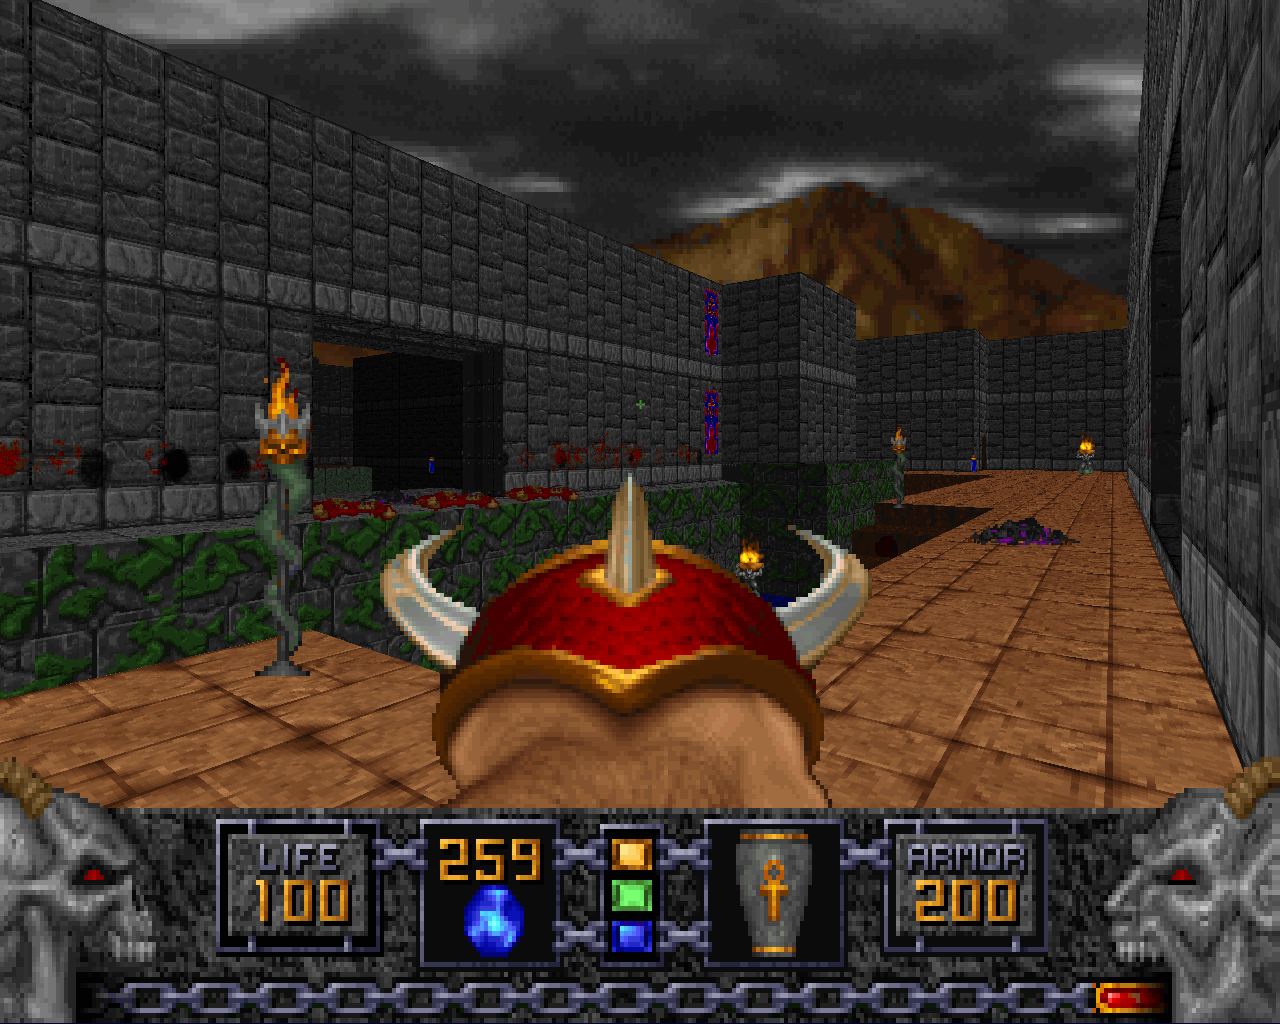
\includegraphics[width=0.8\textwidth]{images/estadodelarte/motores/heretic}
    \caption{\citegame{heretic}, es un juego desarrollado con el motor de Doom (Fuente: doom.wikia.com).}
    \label{heretic}
\end{figure}

Este concepto inició las comunidades de ``modding'', que son grupos de aficionados que desarrollaban juegos nuevos modificando juegos antiguos, y para finales de los noventa, juegos como \citegame{Quake_3} y \citegame{unreal} habían sido diseñados pensando en la reusabilidad de su código. Actualmente, la mayor parte de las compañías desarrolladoras de juegos adquieren la licencia de motores desarrollados por terceros, mucho más económico que desarrollar desde cero todos los componentes.

La línea que separa el motor del juego suele ser difusa y \textbf{depende en gran medida del juego concreto}. El principal factor que se utiliza para distinguir un motor de juego de un juego que haya sido desarrollado de forma ``íntegra'' es la presencia de una arquitectura orientada a datos. Se trata de un paradigma de programación que se basa en diseñar software con la intención de procesar datos, en lugar de en ejecutar secuencias instrucciones fijas.

Idealmente, debería ser capaz de ``reproducir'' cualquier juego a partir de los datos de su contenido, de la misma forma que un programa reproductor de música lee y reproduce canciones. Sin embargo, en la realidad los motores de juegos suelen estar \textbf{optimizados para un determinado género juego o una plataforma especifica} debido a que de esa forma es posible obtener software más eficiente y con mayores prestaciones, aplicando técnicas y patrones de diseño específicos de esos géneros/plataformas.

\subsubsection{Componentes de un Motor}
Los motores de juego son softwares muy complejos, por lo que suelen estar construidos a partir de módulos independientes, lo que facilita enormemente su mantenimiento. Normalmente, un motor de juegos se compone de los siguientes módulos \cite{game_engine_architecture}:
\begin{itemize}
\item\textbf{El núcleo}: Se trata de una aplicación compleja que recoge gran cantidad de herramientas y utilidades necesarias para el desarrollo del juego. El núcleo suele incluir una librería de funciones matemáticas, herramientas para la gestión eficiente de memoria, estructuras de datos y clases personalizadas, etc.
\item\textbf{Motor de renderizado}: Posiblemente el componente más grande y complejo del juego, el motor de renderizado es el software encargado de generar los gráficos del juego. Estos motores suelen estar construidos siguiendo una estructura de capas: primero el \textbf{render de bajo nivel}, que se encarga de dibujar primitivas a la mayor velocidad posible; el \textbf{grafo de escena} determina que sección de la escena es visible, lo que permite reducir el número de llamadas al render de bajo nivel; la capa de \textbf{efectos visuales}, que contiene el sistema de partículas, los efectos de pantalla completa, o las luces dinámicas; y finalmente la capa de \textbf{frontend}, la cual sirve para el renderizado de imágenes 2D que se superpondrán a la escena tridimensional del juego, como los menús, el HUD (Head Up Display) o videos pre-renderizados. Aparte del motor gráfico, los motores de juego actuales suelen incluir también un \textbf{sistema de animación}, el cual permita dotar de movimientos naturales a los personajes y elementos del juego. 
\item\textbf{Gestor de recursos}: Se trata de una interfaz que permite un acceso unificado a los distintos assets que forman el juego (modelos, texturas, sonidos, scripts...). 
\item\textbf{Motor de Físicas}: El motor de físicas permite realizar la detección de colisiones entre entidades del juego, así como la simulación de comportamientos físicos realistas para dichas entidades. Hoy en día, las compañías no suelen programar sus propios motores de físicas, en su lugar adquieren motores desarrollados por terceros, como \textit{Havok}\footnote{https://www.havok.com/physics/} o \textit{PhysX}\footnote{https://www.geforce.com/hardware/technology/physx\#source=gss}.
\item\textbf{Entrada y salida del jugador}: Este sistema se encarga de gestionar la información de entrada del jugador, suministrada mediante el mando de juego o el teclado y ratón. El sistema toma la información en bruto de entrada y permite al programador acceder a ella de forma más útil, limpiando los datos de entrada, creando eventos de activación de teclas y proveyendo de sistemas para mapear funciones a distintas teclas o botones y para detectar secuencias de pulsaciones. Este sistema también provee funciones para la salida de datos relacionado con los mandos de control, como activar y desactivar la vibración o emitir sonidos.
\item\textbf{Sistema de audio}: Es el componente encargado de la reproducción de la música y efectos de sonido del juego. Aunque su complejidad depende en gran medida de las necesidades del motor concreto, la mayoría incluyen sistemas para producir efectos como sonido 3D o música dinámica.
\item\textbf{Networking}: Son los sistemas encargado de realizar la conexión del juego con Internet para, en la mayoría de los casos, realizar partidas en línea con otros jugadores. El soporte de sistemas para el jugo multijugador tiene un gran impacto en la mayoría de los componentes del motor, por lo que estos suelen ser desarrollados pensando desde el principio en el modo multijugador, e implementando el modo de un jugador como un caso específico del multijugador.
\item\textbf{Fundamentos de la jugabilidad}: Esta capa implementa una serie de sistemas que permiten implementar la Jugabilidad. Suele incluir un lenguaje de Scripting, un sistema de eventos, inteligencia artificial, cámaras...
\item\textbf{Herramientas de depuración}: Estas herramientas facilitan la tarea de depurar y optimizar el juego. Incluyen herramientas para dibujar en pantalla, consolas de comandos, sistemas para grabar y reproducir sesiones de juego...
\end{itemize}

\subsection{Ejemplos de Motores}
\subsubsection{Unreal Engine}
El \textbf{Unreal Engine}\footnote{https://www.unrealengine.com/} es un popular motor de juego desarrollado por la compañía Epic Games. Originalmente desarrollado como motor propietario para el juego \citegame{unreal} (figura \ref{unreal-original}), Epic Games pronto empezó a cerrar tratos con otras compañías que querían utilizar el motor en sus proyectos. Actualmente el motor se encuentra en su \textbf{versión 4} y es uno de los más populares del sector, habiendo ganado incluso el premio Guinness al ``motor de juegos más exitoso''\footnote{http://www.guinnessworldrecords.com/world-records/most-successful-game-engine} con un total 408 juegos (a fecha de julio de 2014) desarrollados con Unreal. 

\begin{figure}[h]
	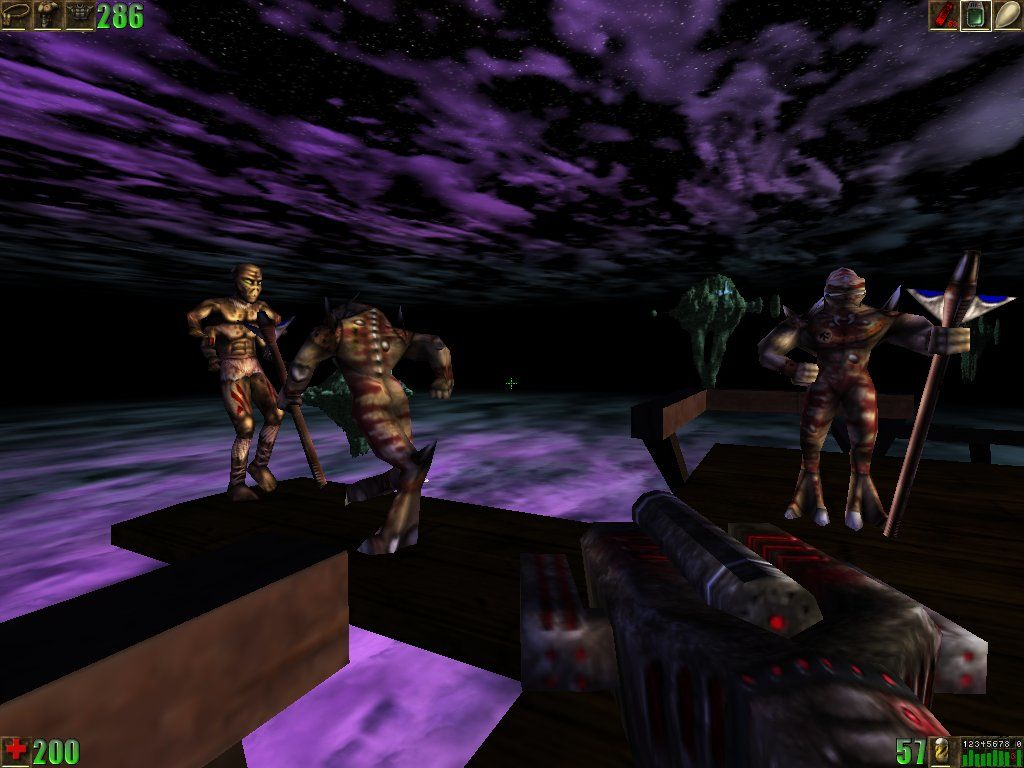
\includegraphics[width=0.85\textwidth]{images/estadodelarte/motores/unreal-original}
    \caption{Unreal (Epic Games, 1998) (Fuente: mobygames.com).}
	\centering
	\label{unreal-original}
\end{figure}

Unreal Engine es un motor orientado al \textbf{desarrollo de juegos AAA}, proyectos de gran envergadura llevados por equipos grandes. Uno de sus puntos fuertes es su potente motor de rendering el cual da soporte a \textbf{gráficos fotorrealistas} y permite el uso de efectos de post-procesados complejos entre otras características. El scripting en Unreal se realiza mediante el sistema \textbf{Blueprint} de scripting visual, el cual permite programar conectando de forma gráfica bloques de código. El motor permite también escribir código directamente en C++, lo que aumenta su flexibilidad. El paquete de herramientas del motor también incluye programas como un editor de escenas (figura \ref{captura-unreal}) generadores de terreno, editores de materiales, herramientas para animación... Sin embargo, se trata de un motor \textbf{complicado y difícil de aprender a utilizar}, además de que la potencia que requiere lo hace poco adecuado para el desarrollo para plataformas móviles.

\begin{figure}[h]
	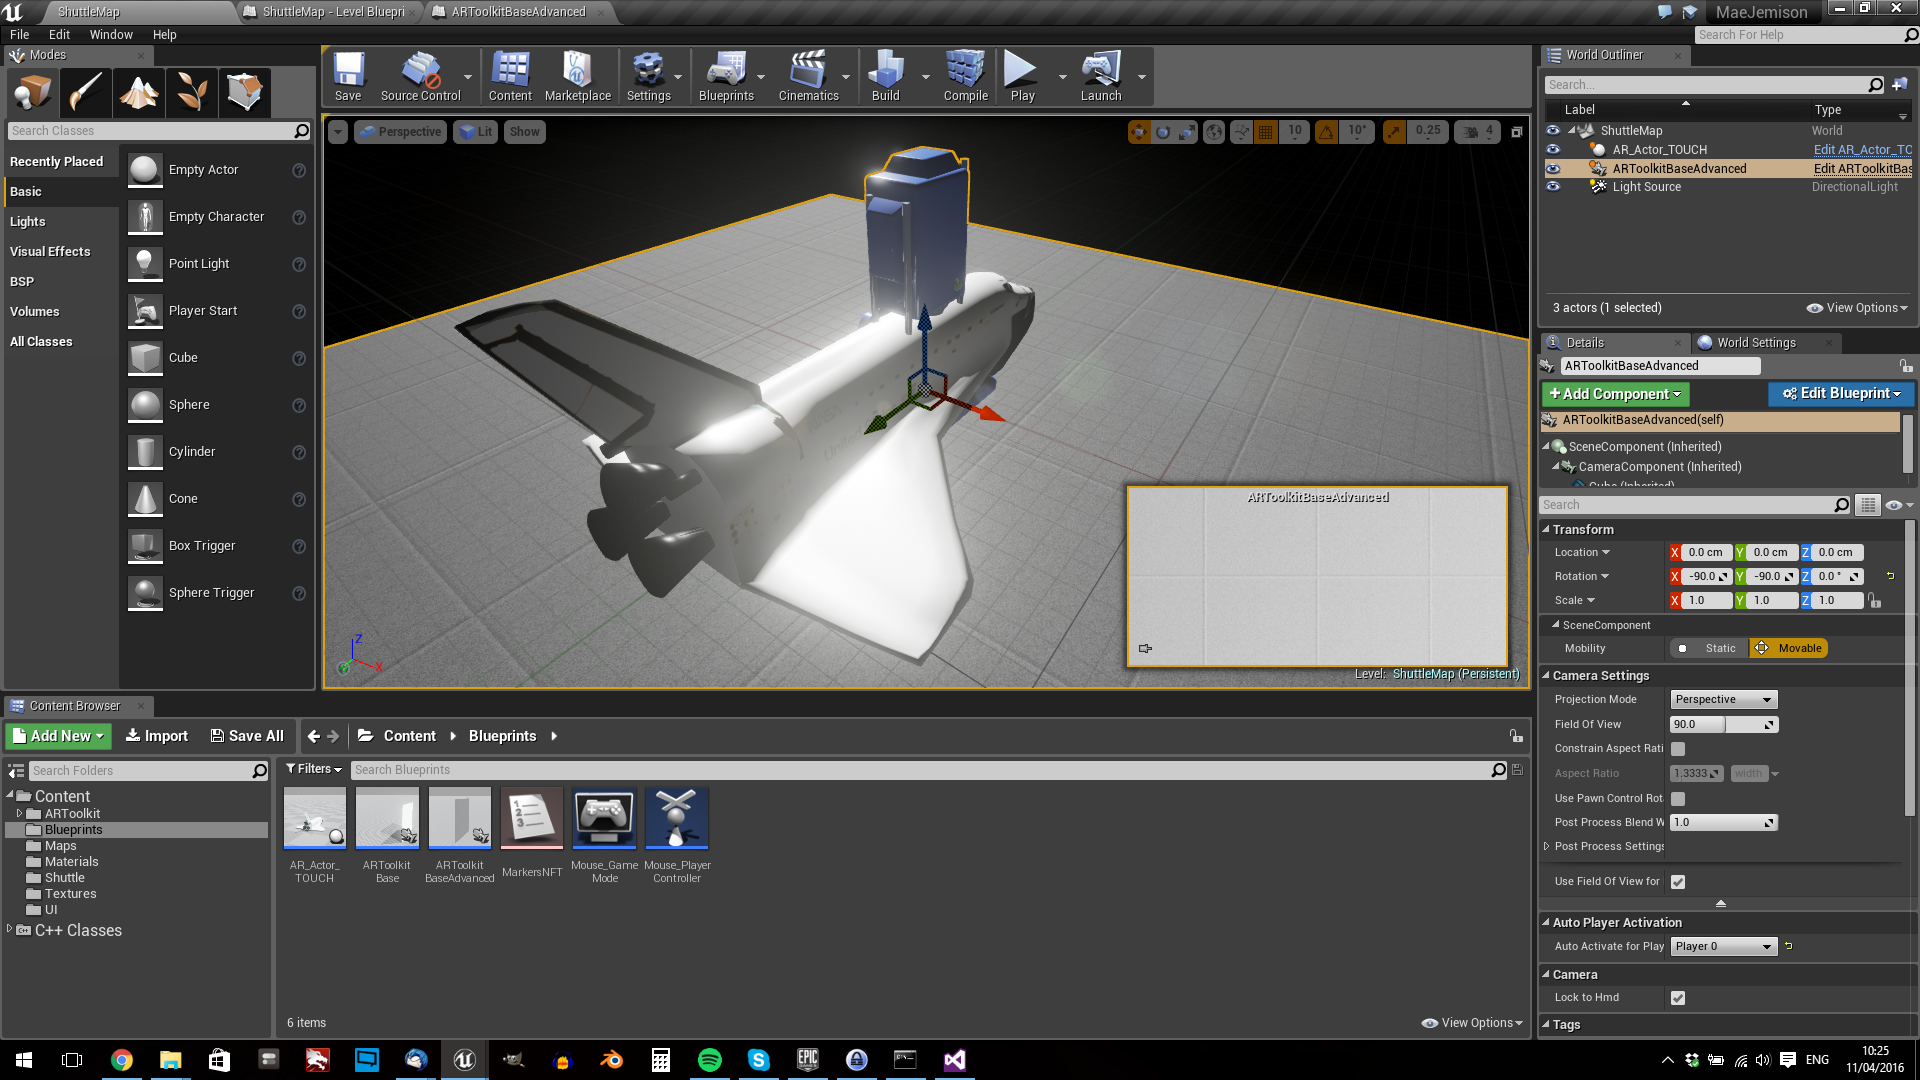
\includegraphics[width=1\textwidth]{images/estadodelarte/motores/captura-unreal}
	\centering
	\caption{Captura del entorno de Unreal Engine (Fuente: docs.unrealengine.com).}
	\label{captura-unreal}
\end{figure}

La licencia de uso de \textbf{Unreal Engine} es gratuita, sin embargo, en proyectos comerciales Epic Games cobra un 5\% de las ganancias a partir de los 3.000\$ por trimestre. En casos especiales, es posible negociar otros tipos de licencias con Epic Games.

\subsubsection{Game Maker Studio}
\textbf{Game Maker Studio}\footnote{https://www.yoyogames.com/gamemaker} es un motor de juegos desarrollado por Yoyo Games. El programa fue lanzado originalmente en 1994 bajo el nombre de \textbf{Amino} como una herramienta para la creación de animaciones. Desde entonces, el programa ha ido evolucionado hasta convertirse en un motor de juegos de calidad profesional.

Game Maker Studio está diseñado para ser muy sencillo de usar: su principal uso es como una herramienta para gente sin conocimientos de programación, para el desarrollo rápido de juegos pequeños o para la creación de prototipos. La interfaz de usuario de su entorno de desarrollo (ver figura \ref{captura-game-maker}) permite la creación de juegos sin escribir ni una sola línea de código, gracias a su sistema\textbf{``Drag and Drop''}, con el que se programa conectando diversos bloques de código. Para el desarrollo de juegos más complejos, el motor ofrece un lenguaje de programación propio llamado \textbf{Game Maker Language}. 

\begin{figure}[h]
	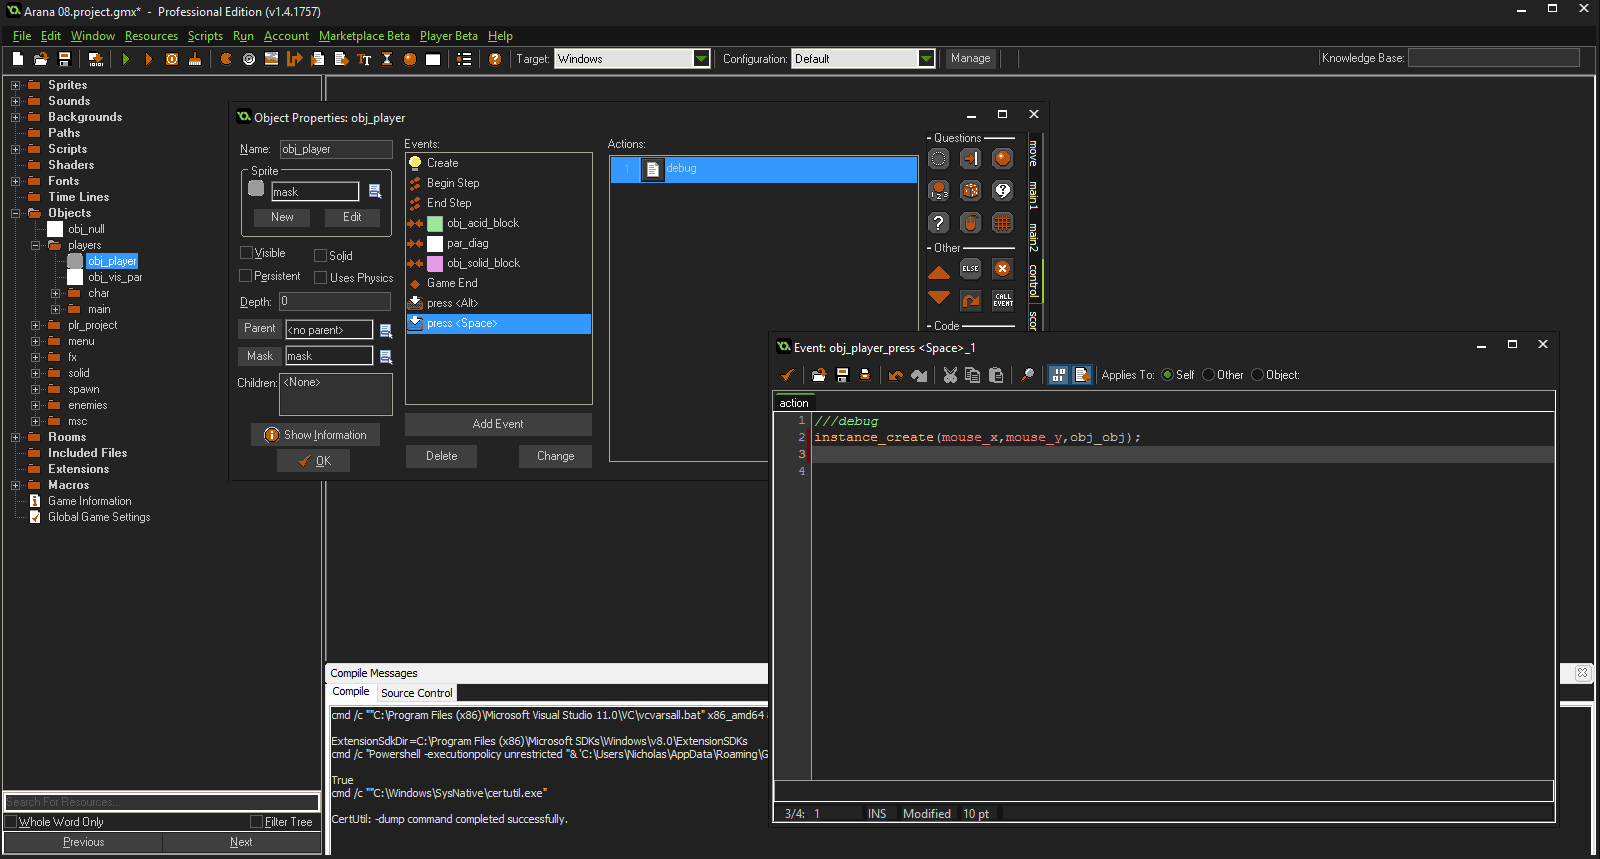
\includegraphics[width=0.8\textwidth]{images/estadodelarte/motores/captura-game-maker}
	\centering
	\caption{Captura del entorno de Game Maker Studio (Fuente: pcgamesn.com).}
	\label{captura-game-maker}
\end{figure}

El motor permite exportar con facilidad a distintas plataformas como PC, dispositivos móviles o HTML5. El entorno integrado de Game Maker incluye herramientas complementarias como un \textbf{editor gráfico} y un \textbf{editor de mapas} para centralizar el desarrollo. Sin embargo, la sencillez del motor también se refleja en su potencia: Game Maker Studio carece de soporte para gráficos tridimensionales complejos, y su arquitectura dificulta el desarrollo de proyectos de gran envergadura. Estas limitaciones no han impedido la creación de juegos exitosos o revolucionarios con este motor, como podría ser \citegame{undertale}, mejor juego de PC del año 2015\footnote{http://www.ign.com/wikis/best-of-2015/PC\_Game\_of\_the\_Year}.

\begin{figure}[h]
	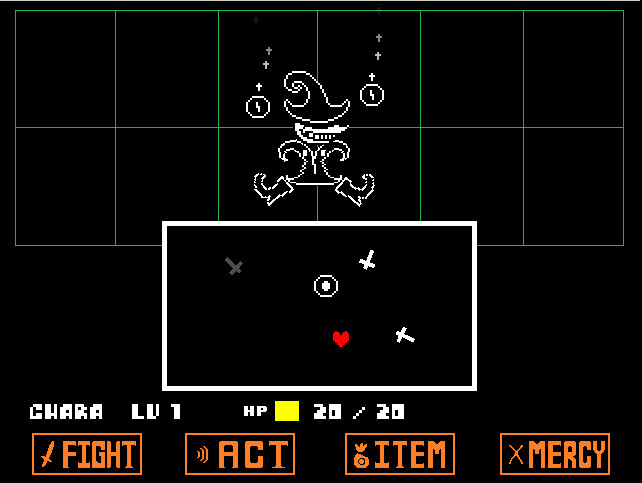
\includegraphics[width=0.8\textwidth]{images/estadodelarte/motores/undertale}
	\centering
	\caption{\citegame{undertale} (Fuente: Página de Steam del juego).}
	\label{undertale}
\end{figure}

La licencia de la versión actual de Game Maker Studio (Game Maker Studio 2) se encuentra a la venta por distintos precios dependiendo de la plataforma de distribución para la que se quiera trabajar: desde la versión básica por 39\$ anuales hasta la versión profesional permanente con posibilidad de exportación a IOS, Android y consolas por 399\$. Existen también una versión de prueba gratuita que cuenta con unas prestaciones reducidas y un plan de pago para su uso en centros educativos.

\subsection{Unity 3D}
\textbf{Unity}\footnote{https://unity3d.com/unity}, conocido popularmente como \textbf{Unity3D}, es un motor de juego multiplataformas diseñado para el desarrollo de videojuegos y otras aplicaciones interactivas tanto en tres dimensiones como en dos dimensiones. Se trata de uno de los motores líderes en el mercado, con más de 170.000 juegos desarrollados con él motor\footnote{https://unity3d.com/sites/default/files/pr\_downloads/bythenumbersunitytechnologies.pdf}, desde pequeños juegos para Android hasta grandes juegos para PC y consolas de sobremesa.

El desarrollo de este motor empezó en el año 2005 de manos de los desarrolladores \textbf{David Helgason, Joachim Ante y Nicholas Francis}. Inicialmente el motor era compatible solo con el sistema operativo Mac OS X, pero ya entonces estaba vigente la filosofía principal del motor: \textbf{una herramienta fácil de usar}, con un sistema de carga de recursos simple y una interfaz completamente gráfica \cite{unity_story}. Con el tiempo, sucesivas versiones del motor fueron desarrolladas para mejorar tanto el rendimiento técnico como su portabilidad a distintos sistemas operativos. Hoy en día (con la versión 2017.5.3), el entorno integrado de desarrollo de Unity es compatible con Windows, Linux y Mac, con posibilidad de exportar juegos a gran variedad de plataformas: desde dispositivos móviles a videoconsolas.

\subsubsection{Características Técnicas}
Unity cuenta con un \textbf{motor de renderizado propietario} de calidad AAA. Se trata de un motor de renderizado basado en físicas que permite la creación de entornos tridimensionales fotorrealistas con iluminación en tiempo real. Adicionalmente, Unity ofrece \textbf{soporte para el uso de gráficos 2D} con el fin de facilitar el desarrollo de juegos de pequeña escala o para dispositivos móviles. El renderizado en Unity se controla mediante shaders escritos en lenguaje Shaderlab, lo que permite al programador escribir sus propios shaders para obtener diversos efectos visuales. 

Para la simulación de las físicas del mundo del juego, Unity ofrece dos motores de físicas, uno para entornos tridimensionales y otro para entornos en 2D. El motor de físicas 3D de Unity es \textbf{PhysX}, desarrollado por NVIDIA, un motor de físicas multiplataformas con soporte para simulación de cuerpos sólidos, tejidos partículas y fluidos. Por otro lado, para la simulación de físicas en entornos bidimensionales Unity utiliza 2D \textbf{Box2D}, un motor de código libre que, si bien cuenta con una funcionalidad más limitada que PhysX, es muy eficiente, ideal para dispositivos móviles y consolas portátiles.

El motor está incluido en un \textbf{entorno de integrado de desarrollo}. La principal característica de este entorno es el llamado \textbf{Editor de Unity} (figura \ref{captura-unity}), una aplicación gráfica en que se encuentra unificada la mayor parte de la funcionalidad necesaria para el desarrollo. El editor incluye una interfaz para la creación y edición de las escenas del juego y los objetos que estas contiene, realiza la gestión de recurso, permite ajustar la configuración... El editor incluye también la función ``play'' que permite iniciar el juego en cualquier momento e incluso realizar cambios en este mientras se encuentra en ejecución.
\begin{figure}[h]
	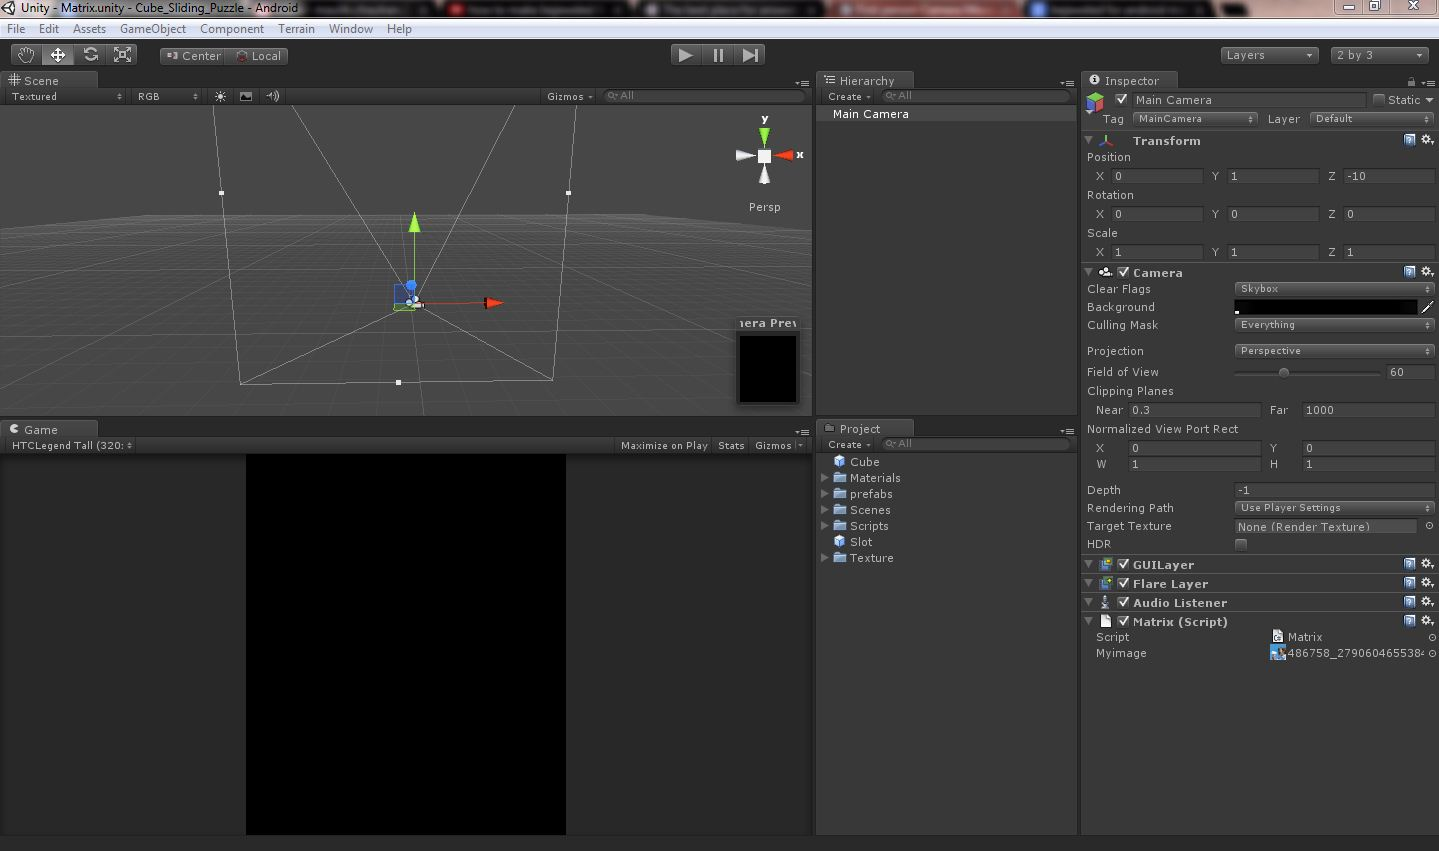
\includegraphics[width=0.8\textwidth]{images/estadodelarte/motores/captura-unity}
	\centering
	\caption{Captura del entorno de desarrollo de Unity (Fuente: answers.unity.com).}
	\label{captura-unity}
\end{figure}

Pero la principal característica del editor de Unity es que es \textbf{completamente personalizable}. Mediante \textbf{scripts de editor}, el programador puede añadir nuevas ventanas, botones e inspectores al editor para así suplirlo de las funcionalidades adicionales que un proyecto dado pueda necesitar. Las librerías para la creación de scripts de editor están integradas con las que el motor utiliza en la implementación del juego, por lo que el programador tiene acceso nativo clases y tipos incluidos de Unity, lo que facilita la creación de herramientas para el desarrollo. Los scripts de editor se guardan como un asset más del proyecto, por lo que el editor puede configurarse individualmente para cada proyecto concreto.

La carga y gestión de \textbf{assets} en Unity es extremadamente sencillas: los recursos se guardan en forma de \textbf{archivos convencionales} dentro de una jerarquía de carpetas dentro del proyecto. Una vez que estos archivos se encuentren dentro de la jerarquía, Unity importara automáticamente cualquier cambio realizado sobre ellos con herramientas externas, lo que agiliza enormemente el desarrollo. Además, Unity cuenta con una tienda en line de recursos para juegos, completamente en el propio editor. Esto permite a los desarrolladores adquirir e integrar fácilmente todo tipo de recursos, desde texturas a sistemas software completos. 

\subsubsection{Programación}
La programación en Unity se realiza mediante \textbf{Scripts}, pequeños programas de código interpretado que se utilizan normalmente para controlar el comportamiento de objetos. Los Scripts de Unity se programan en \textbf{C\#}, un lenguaje de programación desarrollado por Microsoft para su plataforma .NET. Se trata de un lenguaje de programación orientado a objetos, con una sintaxis derivada de C, pero con un proceso de compilación mucho más rápido y flexible. Además de C\#, los scripts de Unity pueden desarrollarse utilizando \textbf{UnityScript}, un lenguaje de programación basado en JavaScript, pero que se encuentra en proceso de ser deprecado en favor de C\#.

Le desarrollo en el entorno Unity es diferente a como se realizaría en un entorno de desarrollo integrado convencional. Esto se debe principalmente a dos factores: en primer el lugar por el énfasis que se hace en el uso del Editor, el cual es necesario para la inicialización y gestión de diversos componentes del juego. En segundo lugar, Unity hace uso de estructuras y clases especificas con las que se debe trabajar, lo que obliga al programador a cambiar su forma de programar.

La clase principal de Unity se llama \textbf{GameObjects}\footnote{https://docs.unity3d.com/ScriptReference/GameObject.html}. Los objetos de esta clase se instancian en el editor de Unity o mediante código con el método estático \textbf{Instantiate}\footnote{https://docs.unity3d.com/ScriptReference/Object.Instantiate.html}, sin embargo, la funcionalidad de los GameObjects viene dada por los objetos de la clase \textbf{Component}\footnote{https://docs.unity3d.com/Manual/Components.html}. Esta clase es padre de multitud de componentes con diferente funcionalidad. Algunos de los componentes más importantes de Unity son los siguientes:
\begin{itemize}
\item \textbf{Transform}\footnote{https://docs.unity3d.com/ScriptReference/Transform.html}: Este componente almacena la posición, rotación y escala del objeto en la escena. Cada transform tiene un padre, lo que permite aplicar las transformaciones de forma jerárquica. Como su función es tan importante, todos los GameObjets tienen uno asociado.
\item \textbf{Collider}\footnote{https://docs.unity3d.com/ScriptReference/Collider.html}: Los colliders son una familia de componentes que permiten realizar la detección de colisiones. Existen muchos tipos de colliders dependiendo de su forma (BoxCollider, SphereCollider...). La clase Collider y sus hijos interaccionan con el motor de físicas 3D de Unity, para las colisiones entre objetos en 2D se utiliza la familia de clases \textbf{Collider2D}.
\item \textbf{Rigidbody}\footnote{https://docs.unity3d.com/ScriptReference/Rigidbody.html}: Esta clase se utiliza para la simulación física de cuerpos rígidos en 3D. Rigidbody contiene métodos para aplicar cambios de posición y rotación a objetos basándose en su velocidad, aceleración, fricción... Para objetos en 2D, existe una clase equivalente llamada \textbf{Rigidbody2D}.
\item \textbf{Renderer}\footnote{https://docs.unity3d.com/ScriptReference/Renderer.html}: Este componente permite renderizar modelos y texturas en la escena. 
\item \textbf{Audio Source}\footnote{https://docs.unity3d.com/ScriptReference/AudioSource.html}: Los audio source son componentes que permiten a los objetos emitir clips sonido. El componente permite aplicar transformaciones en tiempo real a los sonidos que emite, como modificar su volumen o la altura de su tono.
\item \textbf{Animator}\footnote{https://docs.unity3d.com/ScriptReference/Animator.html}: Este componente permite añadir animaciones a los objetos. Se trata de una máquina de estados finitos que reproduce clips de animación de forma condicional. Estos clips pueden producir variaciones en las propiedades de otros componentes del objeto en función del tiempo.
\item \textbf{Particle System}\footnote{https://docs.unity3d.com/ScriptReference/ParticleSystem.html}: Es un componente que emite \textbf{partículas}, pequeñas imágenes 2D que permiten crear efectos visuales como fuego o explosiones.
\end{itemize}

El programador puede crear sus propios componentes (llamados \textbf{Scripts} extendiendo la clase \textbf{MonoBehaviour}\footnote{https://docs.unity3d.com/ScriptReference/MonoBehaviour.html}. Esta clase, hija de la clase Component, provee de una serie de métodos especiales llamados \textbf{Eventos} los cuales son llamados automáticamente por Unity en momentos clave de la ejecución. Algunos de estos eventos son \textbf{Start}, que es llamado al principio de la ejecución; \textbf{Update}, que se ejecuta una vez por fotograma o \textbf{OnCollision} al que se llama cuando el objeto colisiona con otro. 

Los GameObject se crean dentro de unas estructuras llamadas \textbf{Escenas}\footnote{https://docs.unity3d.com/Manual/CreatingScenes.html}. Cada escena contiene un entorno o menú del juego en forma de archivo, así es posible organizar mejor las distintas secciones del juego completo. Normalmente solo una escena se encuentra activa al mismo tiempo, pudiéndose cambiar por otra tanto en el editor como en tiempo de ejecución, pero es posible cargar múltiples escenas al mismo tiempo.

\subsubsection{Licencia y Plataformas}
Unity es un programa de \textbf{código cerrado}, para poder utilizarlo es necesario adquirir la licencia de manos de Unity Technologies. Existen distintos tipos de planes de pago a la hora de adquirir la licencia, estos son:
\begin{enumerate}
\item\textbf{Licencia Personal}: Esta licencia está pensada para usuarios amateur o estudiantes. La licencia incluye acceso a toda la funcionalidad del motor junto con ciertos plugins como sistemas de publicidad y pago en la aplicación. Sin embargo, esta licencia no puede ser adquirida por ninguna entidad que más de 100.000\$ anuales, viéndose obligada a adquirir alguna de las otras licencias. Esta licencia es totalmente gratuita. 
\item\textbf{Licencia Plus}: Esta licencia está pensada para estudios pequeños. Junto con toda la funcionalidad de la licencia personal, esta licencia incluye herramientas para gestionar métricas del juego y realizar estudios de rendimiento exhaustivos. Esta licencia también tiene una cifra de beneficios máxima, obligando a sus usuarios a adquirir la licencia pro si se superan los 200.000\$ de beneficio anuales. El precio de esta licencia es de 35\$ anuales.
\item\textbf{Licencia Pro}: Es la licencia para grandes estudios. Esta versión de la licencia cuenta con un mejor soporte para juegos multijugador, un mejor sistema para realizar análisis de métricas y acceso anticipado a las nuevas características, junto con toda la funcionalidad de las licencias anteriores. El precio de esta licencia es de 125\$ al mes.
\end{enumerate}

Todas las licencias incluyen el editor de Unity con soporte para \textbf{Windows, Linux y Mac OS}. Independientemente de la plataforma de desarrollo elegida, Unity permite la exportación a más \textbf{20 plataformas distintas}: Dispositivos móviles (tanto Android como IOS), ordenadores de sobremesa, videoconsolas de última generación y web. Unity incluye herramientas para facilitar la conversión entre distintas plataformas. Juegos desarrollados con Unity como \citegame{pacman_256} (figura \ref{pacman-256}) están disponibles en múltiples plataformas gracias a esta característica.
\begin{figure}[h]
	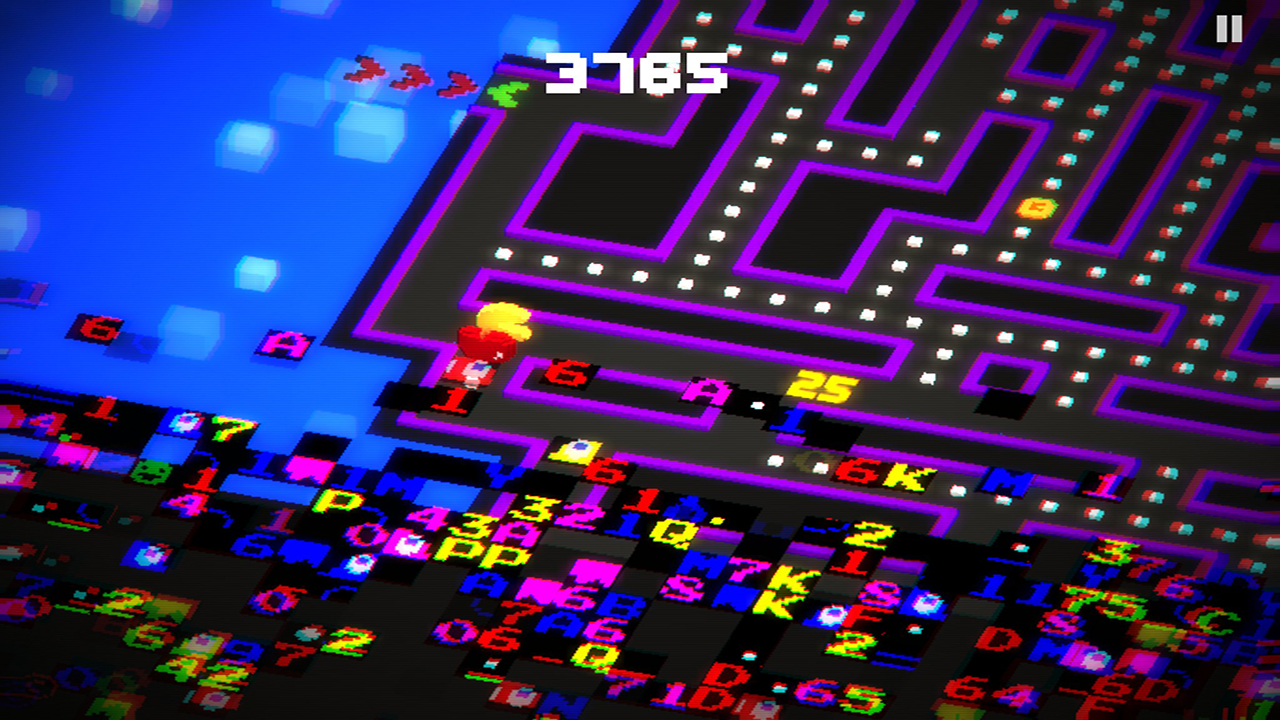
\includegraphics[width=0.8\textwidth]{images/estadodelarte/motores/pacman-256}
	\centering
	\caption{\citegame{pacman_256}, disponible para PC, Android, IOS, PS4 y XBOX One (Fuente: página de Steam del juego).}
	\label{pacman-256}
\end{figure}

\section{Inteligencia Artificial en Videojuegos}
\subsection{Historia}
Desde los principios de la inteligencia artificial, los expertos han dedicado una importante cantidad de tiempo y esfuerzo para construir sistemas inteligentes con el propósito de que pudiesen jugar a juegos con un nivel igual o superior al humano. Este enfoque en el estudio de los juegos se debe a que \textbf{ofrecen un campo de estudio ideal para la inteligencia artificial}: los juegos son problemas complejos que ofrecen desafíos para múltiples campos de la inteligencia artificial y además son tan populares que se dispone de cantidades inmensas de información sobre ellos \cite{ai_and_games}.

Los primeros programas capaces de jugar contra humanos surgieron en los años cincuenta. Uno de los ejemplos más antiguos es el algoritmo ajedrecista de \textbf{Alan Turing} de 1948 \cite{turing_chess}, el cual era ``ejecutado'' en papel por un humano que seguía manualmente los pasos del algoritmo. El primer Software capaz de jugar a un jugo fue la inteligencia artificial para el juego \citegame{oxo}. En 1959, \textbf{Arthur L. Samuel} \cite{machine_learning} programó una inteligencia artificial para jugar a las Damas la cual contaba con un sistema de aprendizaje y jugaba a nivel \textit{amateur} \cite{ia_moderno}. 

Sin embargo, estos programas eran muy simples y no planteaban reto alguno contra jugadores experimentados cuando se trataba de juegos con una cierta complejidad, como el ajedrez. Hubo que esperar a los años noventa para que empezaran a surgir programas capaces de derrotar a grandes maestros de distintos juegos: en el año 1994 el programa \textbf{Chinook Checkers} derrotó al campeón mundial de la Damas \textbf{Marion Tinsley}\footnote{https://webdocs.cs.ualberta.ca/~chinook/project/} y 3 años más tarde el super-ordenador \textbf{Deep Blue} venció a gran maestro del ajedrez \textbf{Gary Kasparov}\footnote{http://www-03.ibm.com/ibm/history/ibm100/us/en/icons/deepblue/} (figura \ref{deepblue-vs-kasparov}). Hoy en día, la inteligencia artificial ha demostrado ser capaz de superar a los jugadores humanos en casi cualquier juego, con ejemplos tales como la inteligencia artificial \textbf{Watson} ganando el concurso de televisión \textbf{Jeopardy} en 2011\footnote{https://www.youtube.com/watch?v=WFR3lOm\_xhE} o el programa \textbf{AlphaGo} derrotando a \textbf{Ke Jie}, el jugador número uno de Go\footnote{https://www.theverge.com/2017/5/25/15689462/alphago-ke-jie-game-2-result-google-deepmind-china} (un juego con una complejidad varios ordenes de magnitud superior al ajedrez).

\begin{figure}[h]
	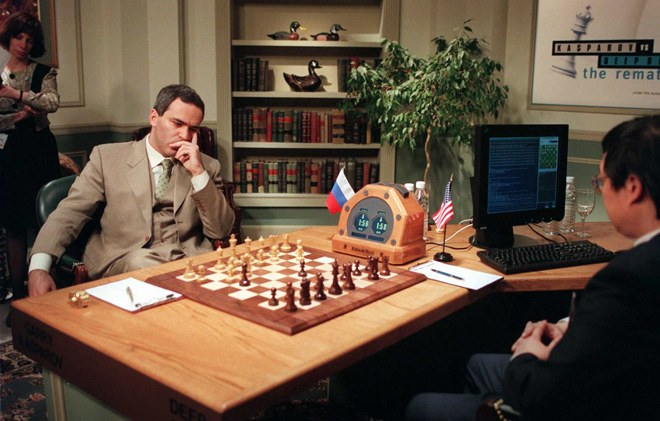
\includegraphics[width=0.8\textwidth]{images/estadodelarte/ai/deepblue-vs-kasparov}
	\centering
	\caption{El Gran Maestro de ajedrez Garri Kaspárov (izquierda) enfrentándose al ordenador Deep Blue (derecha).}
	\label{deepblue-vs-kasparov}
\end{figure}

Hoy en día, con el auge de los videojuegos, ha comenzado el estudio para la resolución de juegos continuos en tiempo real (en contraste a los juegos de mesa tradicionales, que son discretos). Estos juegos presentan un desafió mayor, pero ya se han realizado avances como el algoritmo desarrollado por \textbf{Google DeepMind} en 2014 para la resolución de varios juegos de la consola clásica Atari 2600\footnote{https://deepmind.com/research/publications/playing-atari-deep-reinforcement-learning/}.

\subsection{IA Aplicada a Videojuegos: Contexto Actual}
El uso de la inteligencia artificial en la industria del videojuego difiere en varios puntos a su aplicación habitual en el campo académico de los juegos. La principal diferencia es el tipo de problema que se intenta resolver utilizando inteligencia artificial en cada una de las ramas: en la inteligencia artificial aplicada a jugar a juegos se busca obtener un sistema capaz de jugar de manera óptima para derrotar a cualquier adversario humano, sin embargo, en la inteligencia artificial orientada a videojuegos lo que se busca es crear sistemas con los que \textbf{mejorar la experiencia de juego del jugador}. Esta diferencia de objetivos hace que la inteligencia artificial no se aplique únicamente a la creación de oponentes virtuales, sino también al modelado del comportamiento de \textbf{personajes no jugadores} y a la \textbf{generación procedimental de contenido} \cite{ai_and_games}.

En el ámbito de los videojuegos, a la Inteligencia Artificial que interacciona con el juego como un jugador más suele llamarse \textbf{bot}. Estos bots predominan en juegos competitivos donde es necesario un oponente con un \textbf{grado de inteligencia elevado} para suponer un reto al jugador, como los juegos de estrategia, los juegos de lucha o los juegos de disparos en primera persona. Debido al elevado coste y complejidad de desarrollar una Inteligencia Artificial potente para estos juegos, por no hablar de la potencia requerida para ejecutarla, en la mayor parte de los videojuegos la inteligencia artificial \textbf{``hace trampas''}, juega teniendo acceso una serie de ventajas que los jugadores humanos no tiene. Estos sistemas podrían, por ejemplo, acceder a información oculta del jugador (como la posición o recursos) a la hora de planificar estrategias o dispondrían de más y mejores recursos que sus adversarios \cite{ai_and_games}.

En la mayoría de los juegos, la inteligencia artificial no se dedica al modelado de bots como los descritos anteriormente, sino que lo más común es que se utilice para controlar el comportamiento de \textbf{personajes no jugadores}, o NPCs (siglas inglesas de Non-Player Character). Estos pueden tener comportamientos muy variados dependiendo de su papel en el juego: pueden actuar como adversarios, servir de ayuda para el jugador, formar parte de un puzle, contar una historia o simplemente formar parte del trasfondo de la acción. Dependiendo de la función asignada, la inteligencia artificial de un NPC puede variar desde una simple torreta que dispara a intervalos regulares hasta complejos sistemas de toma de decisiones como en \citegame{sims} (figura \ref{sims-captura})
\begin{figure}[h]
	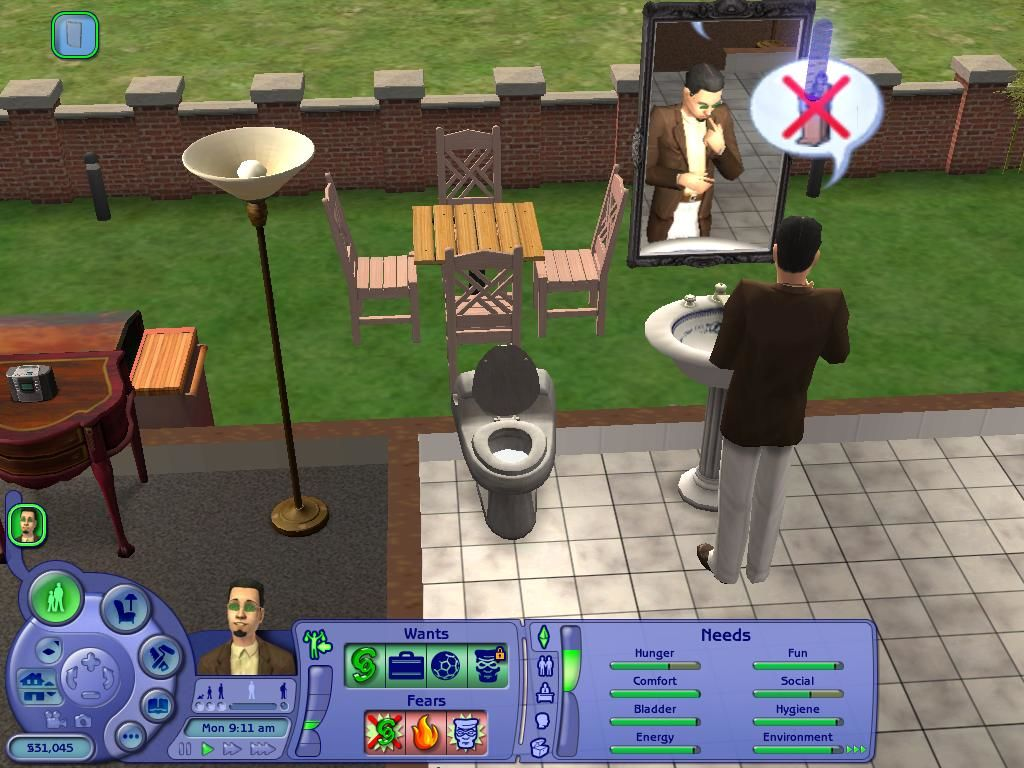
\includegraphics[width=0.8\textwidth]{images/estadodelarte/ai/sims-captura}
	\centering
	\caption{En \citegame{sims}, los personajes pueden tomar decisiones basándose en sus gustos y necesidades.}
	\label{sims-captura}
\end{figure}

Los NPCs en videojuegos se diseñan con dos objetivos en mente. En primer lugar, se busca crear una \textbf{ilusión de inteligencia}, de forma que los jugadores crean que el NPC es un ser inteligente con un comportamiento creíble, para que le resulte más fácil sentirse \textbf{inmerso} en la acción del juego. En segundo lugar, él debe buscarse hacer que el propio jugador se sienta inteligente al interaccionar con los NPCs. Esto se logra, especialmente cuando se trata de adversarios, haciendo que su comportamiento sea hasta cierto punto \textbf{predecible}, de forma que el jugador pueda desarrollar estrategias para enfrentarse/interaccionar con ellos \cite{ia_moderno}. 

La otra aplicación principal en los videojuegos es la \textbf{Generación Procedimental de Contenido}. La generación procedimental de contenido es el nombre que reciben los métodos que permiten generar el contenido de un juego de forma automática o con solo un mínimo de intervención humana. Actualmente, la mayor parte de los juegos que hacen uso de la generación procedimental la utilizan para la \textbf{creación automática de mapas} (como en el caso de \citegame{minecraft} (ver figura \ref{minecraft})) u objetos (como por ejemplo en \citegame{diablo_2}). La generación procedimental de contenido puede utilizarse tanto como una \textbf{herramienta durante el desarrollo}, que serviría para generar contenido que luego sería refinado por los desarrolladores; o podría formar parte del juego final, generando nuevo contenido al gusto del jugador de forma automática \cite{ai_and_games}.

\begin{figure}[h]
	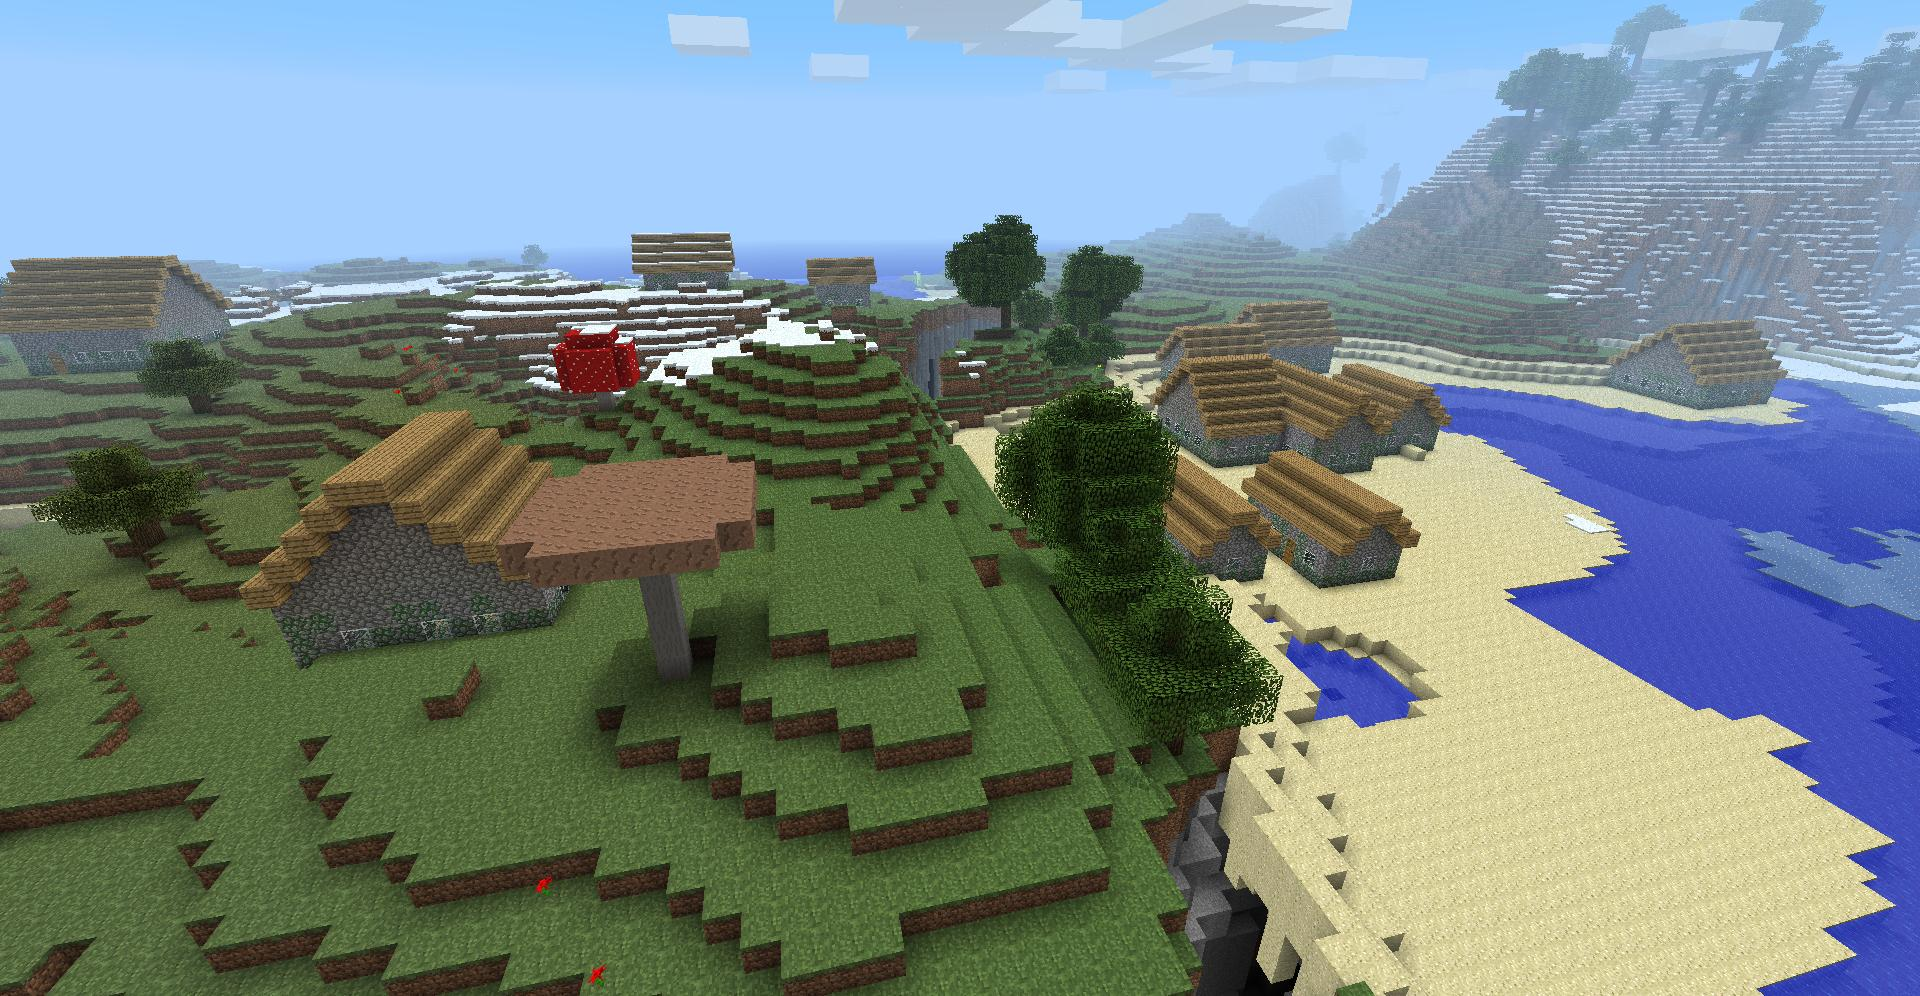
\includegraphics[width=0.8\textwidth]{images/estadodelarte/ai/minecraft}
	\centering
	\caption{\citegame{minecraft} es un ejemplo claro de generación procedimental de terrenos.}
	\label{minecraft}
\end{figure}

\subsection{Métodos de la IA}
Existen varios tipos de métodos y algoritmos los cuales pueden ser utilizados para construir inteligencias Artificiales. La elección entre los distintos tipos de métodos debe realizarse dependiendo del tipo de problema que se intenta resolver y de los recursos de los que se dispone, tanto las prestaciones del dispositivo en el que van a ser implementados como margen de tiempo máximo de la ejecución del algoritmo \cite{ai_and_games}. 

Los Métodos de la inteligencia artificial pueden ser agrupados en las siguientes categorías, debido a sus características y aplicaciones similares:

\subsubsection{Métodos Ad Hoc}
Esta clase de métodos de IA es una de la primera y, en el sector del videojuego, la más común. Su nombre proviene de la locución latina que, traducida, significa ``para esto'', y hace referencia a que se tratan de \textbf{soluciones precisas para problemas concretos}, las cuales no pueden generalizarse ni aplicarse a otros problemas distintos \cite{ai_and_games}.

Pese al notable problema que provoca la falta de reusabilidad de estos métodos, son los más utilizados en el desarrollo de videojuegos. Esto se debe a que, por lo general, son muy fáciles de diseñar, visualizar, implementar y depurar; además requerir de muy pocos recursos cuando se aplican a problemas pequeños.

El primero de estos métodos son las \textbf{máquinas de estados finitos} o FSM por sus siglas en inglés, el método dominante en la industria para el desarrollo de  artificiales hasta mediados de los 2000 \cite{ai_and_games}. Este método se basa en dividir el comportamiento de la inteligencia artificial en varios \textbf{estados} independientes, cada uno con su propia lógica. Estos estados se encuentran conectados mediante \textbf{transiciones} las cuales cambian de un estado a otro si se cumplen determinadas condiciones.

\begin{figure}[h]
	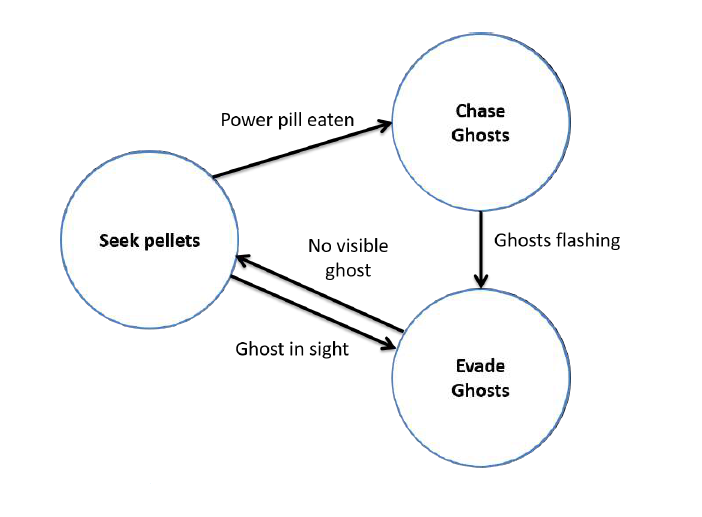
\includegraphics[width=0.8\textwidth]{images/estadodelarte/ai/pacman-fsm}
	\centering
	\caption{FSM de alto nivel de una IA jugadora de \citegame{pacman} (figura extraída de \cite{ai_and_games}).}
	\label{pacman}
\end{figure}

La implementación de las máquinas de estados es \textbf{tremendamente simple, son fáciles de depurar, intuitivas y muy flexibles}, pudiéndose aplicar incluso a problemas no relacionados con la inteligencia artificial como la gestión de menús del juego \cite{libro_esi}. Sin embargo, su complejidad escala muy rápido con problemas grandes y además tienden a ser muy previsibles al carecer de capacidad de adaptación \cite{ai_and_games}.

Una evolución directa de las máquinas de estados son los \textbf{árboles de comportamiento}. Este tipo de Inteligencias Artificiales ejecutan una secuencia de \textbf{comportamientos}, los cuales se encuentran ordenados en una estructura en árbol. El programa recorre el árbol en profundidad, ejecutando los comportamientos por los que pasa. Si la ejecución del comportamiento es \textit{exitosa}, se prosigue con la ejecución, pero si es un \textit{fallo} entonces se reinicia la ejecución \cite{ai_and_games}. Aparte de los comportamientos, los arboles de comportamiento incluyen otros tres tipos de nodos:
\begin{itemize}
\item \textbf{Secuencia}: Este nodo ejecuta en secuencia el comportamiento de sus nodos hijos. Su ejecución será exitosa si lo fue la de todos sus nodos hijos.
\item \textbf{Selector}: Este nodo selecciona de entre sus nodos hijos uno para ejecutar, basándose en algún tipo de filtro (los más comunes son los probabilistas o los basados en prioridad). Si falla la ejecución del hijo seleccionado, se puede elegir otro hijo o devolver un fallo.
\item \textbf{Decorador}: Este tipo de nodo añade modificaciones a la ejecución de su nodo hijo. Las más habituales son las que repiten la ejecución mientras se cumpla cierta condición (tiempo transcurrido, número de ejecuciones...).
\end{itemize}

Los arboles de comportamiento \textbf{son mucho más flexibles} que las máquinas de estados, ya que es mucho más sencillo añadir y quitar comportamientos. Además, elementos como los nodos selectores probabilistas permiten diseñar mucho más predecibles. Este tipo de inteligencia artificial ya ha sido implementada en varios títulos comerciales como \citegame{bioshock} o \citegame{halo_2}\footnote{https://www.gamasutra.com/view/feature/130663/gdc\_2005\_proceeding\_handling\_.php}.

El método Ad Hoc más reciente se llama \textbf{inteligencia artificial basada en Utilidad}. La idea principal de este método es que cada posible acción o estado de la inteligencia artificial tiene asignado un \textbf{valor de utilidad}, que representa como de útil es dicha acción o estado dada la situación actual del sistema. La utilidad se calcula a partir de la combinación de uno o varios \textbf{factores de decisión}, variables que representan el estado del mundo del juego.\cite{gameaipro}.

Gracias a la facilidad para la creación de nuevos factores de decisión, y la facilidad para asociarlos con la utilidad, este método es mucho más \textbf{modular y extensible} los métodos Ad Hoc anteriormente mencionados. Se trata de una técnica relativamente nueva en la industria, por lo que su uso aún no está muy extendido.

\subsubsection{Algoritmos de búsqueda}
Una de las bases de la inteligencia artificial son los \textbf{algoritmos de búsqueda}, dado que la mayor parte de los problemas de la inteligencia artificial podrían plantearse usando este tipo de algoritmos \cite{ai_and_games}. Los algoritmos de búsqueda se basan en, dado un \textbf{problema} y un \textbf{estado inicial}, encontrar una secuencia de acciones que permitan alcanzar la \textbf{solución} del problema partiendo del estado inicial

Para encontrar la solución del problema, los algoritmos de búsqueda hacen uso de \textbf{árboles de búsqueda}, un tipo de grafo dirigido en el cual los \textbf{nodos} o hojas representan estados del problema, mientras que las \textbf{aristas} o ramas representan las acciones que provocan la transición entre dos estados. El agente inteligente recorre el árbol partiendo del \textbf{nodo raíz} (el estado inicial) buscando la secuencia de ramas que lleven a la solución del problema \cite{ia_moderno}. 

Partiendo de esta base, existen numerosos algoritmos de búsqueda distintos, los cuales utilizan diferentes estrategias a la hora de escoger de entre los distintos nodos del árbol cual debe ser analizado. Dependiendo del tipo de estrategia de selección, los algoritmos de búsqueda pueden agruparse en las siguientes categorías:
\begin{itemize}
\item \textbf{Búsqueda no informada}: Se trata de los algoritmos más básicos, en los que se realiza la búsqueda sin ningún tipo de información adicional sobre el objetivo. Sus variantes más simples son el algoritmo \textbf{primero en anchura}(explora todas las acciones de un estado antes de pasar al siguiente) y el \textbf{primero en profundidad} (explora una secuencia de ramas todo lo que puede antes de volver e intentar otra secuencia distinta)
\item \textbf{Búsqueda primero el mejor}: En estos algoritmos se cuenta con información adicional sobre el nodo objetivo, la cual se utiliza para determinar que nodos deben explorarse primero. Un tipo de algoritmos Primero el Mejor son los algoritmos \textbf{A*}, en los cuales los nodos se seleccionan basándose en su \textbf{coste} (suma de la distancia entre el nodo y el nodo raíz y la distancia estimada al objetivo.
\item \textbf{Búsqueda MiniMax}: Este tipo de algoritmos se utilizan para resolver problemas que involucran a dos adversarios enfrentados. En estos algoritmos se va alternando entre jugadores \textbf{min y max}, los cuales intentan llegar a sus respectivos estados de victoria opuestos. El espacio de búsqueda de estos algoritmos suele ser muy grande, por lo que suelen usar funciones de evaluación para evitar recorrer el árbol de búsqueda completo.
\item \textbf{Árbol de búsqueda de Monte Carlo}: Se trata de una familia de algoritmos diseñados para resolver problemas \textbf{No deterministas} y/o de \textbf{Información Imperfecta}. Para evaluar la calidad de un estado dado, el algoritmo utiliza simulaciones aleatorias de partidas a partir de ese estado. La siguiente acción será con la que empezó el mayor número de partidas victoriosas.
\end{itemize} 

Cuando se aplican a juegos, los arboles de búsqueda suelen aplicarse para resolver dos tipos de problemas: para la búsqueda de caminos y para resolver juegos basados en turnos discretos.

\subsubsection{Algoritmos de Optimización}
Los \textbf{algoritmos de optimización}, a diferencia de la búsqueda en árbol, se centran en obtener una solución correcta, ignorando los pasos que llevaron a esta. Para ello, el algoritmo empieza tomando una solución sub-optima, la cual va modificando en múltiples iteraciones utilizando una \textbf{función de Aptitud} como guía hasta obtener una solución con una Aptitud máxima\cite{ai_and_games}.

Existen varios tipos de algoritmos de optimización, dependiendo de los métodos que elijan para la selección de la solución inicial, para la evaluación de aptitud o para la modificación:
\begin{itemize}
\item \textbf{Búsqueda local}: Este tipo de algoritmos consisten en, dada una solución, revisar todas las soluciones que difieran de dichas soluciones por una distancia mínima. Si alguna de las soluciones mejora a la solución original, se remplaza la solución original por la nueva solución y repite el algoritmo; si no, la solución original es elegida como la solución óptima.
\item \textbf{Algoritmos evolutivos}: Los algoritmos evolutivos son un tipo de algoritmos de optimización basados en la evolución por \textbf{selección natural Darwiniana} que se observa en la naturaleza. Su funcionamiento se basa en un conjunto amplio de soluciones candidatas. EN cada iteración del algoritmo, las distintas soluciones se ``cruzan'' para obtener soluciones mixtas, las cuales son evaluadas. Finalmente, se forma un nuevo conjunto de soluciones a partir de las soluciones más exitosas. El algoritmo se repite hasta obtener la solución óptima.
\end{itemize} 

\subsubsection{Aprendizaje Automático}
El aprendizaje automático es una rama de la computación que permite dotar a los ordenadores de la capacidad de \textbf{aprender} a realizar una tarea utilizando datos en lugar de programarlo específicamente para esa tarea \cite{machine_learning}. Los algoritmos de aprendizaje automático suelen aplicarse a problemas donde es muy difícil, o incluso imposible, programar un algoritmo implícito que pueda resolverlo, como por ejemplo el filtrado de correos o la visión por ordenador.

Una forma de clasificar los algoritmos de aprendizaje automático es basándose en el tipo de \textbf{Retroalimentación} que reciben. De esta forma, surgen las siguientes categorías:
\begin{itemize}
\item \textbf{Aprendizaje supervisado}: Se trata de algoritmos que extraer los atributos y características comunes de los integrantes de grupos etiquetados. Estos algoritmos funcionan recibiendo conjuntos de muestra formado por datos etiquetados en distintos grupos y categorías. Analizando los conjuntos de muestra, el algoritmo debe ser capaz de asignar nuevos datos a la categoría correcta. Existen muchos tipos de algoritmos de Aprendizaje supervisado, como por ejemplo las \textbf{Redes Neuronales}, que funcionan imitando la estructura de las neuronas del cerebro.
\item \textbf{Aprendizaje por refuerzo}: Los algoritmos de aprendizaje por refuerzo se inspiran en el \textbf{conductismo psicológico}, basándose en la forma en la que los animales aprenden a tomar decisiones basándose en los estímulos positivos y negativos de su entorno. Estos algoritmos suelen implementarse mediante un agente inteligente que interacciona con un entorno mediante acciones. Con cada acción, el agente recibe un estímulo positivo o negativo, que almacena con la intención de descubrir la secuencia de acciones que maximice el estímulo positivo a largo plazo mediante técnicas similares a los algoritmos de optimización
\item \textbf{Aprendizaje no supervisado}: El aprendizaje no supervisado son un conjunto de algoritmos que sirven para encontrar asociaciones y patrones en un conjunto de datos sin ningún tipo de información de refuerzo adicional. Existen varias aproximaciones a este tipo de algoritmos, como el \textbf{clustering}, que consiste en agrupar elementos de un conjunto basándose en su similitud entre ellos y su diferencia con el resto de los grupos.
\end{itemize} 

La principal limitación del aprendizaje automático es la necesidad de convertir los datos de entrada a \textbf{representación de datos} interna que permita al algoritmo encontrar y clasificar los patrones correctamente. Ante la dificultad de elaborar las representaciones de ciertos tipos de información (como imágenes o el lenguaje natural) surgieron los algoritmos de \textbf{Deep Learning}, métodos de aprendizaje automático especializados en el aprendizaje de modelos de representación.

Los algoritmos de deep learning se caracterizan por utilizar \textbf{múltiples capas de unidades de procesamiento}. Cada capa recibe unos datos de entrada que procesa para generar convertirlos en un sistema de representación de más alto nivel, los cuales serán usados como entrada en la siguiente etapa. La estructura de capas no está diseñada por un ingeniero humano, sino que son generadas utilizando algoritmos de aprendizaje automático de propósito general, el cual puede ser tanto supervisados como no supervisados cite \cite{deep_learning}. 

\subsection{Futuros campos de aplicación}
La inteligencia artificial orientada a juegos evoluciona de manera paralela a los propios videojuegos, que viven ahora más que nunca una época dorada debido al aumento constante tanto en popularidad y prestigio, lo que supone una mejora tanto en la potencia de las máquinas que los ejecutan como en las técnicas que se utilizan en su desarrollo. Esta situación cambiante ha causado la aparición de nuevos problemas que se esperan poder solucionar con el uso de técnicas de inteligencia artificial \cite{ai_and_games}.

Una las posibles aplicaciones de la inteligencia artificial es la de realizar \textbf{testing de juegos}. El programa jugaría a los juegos en busca de fallos tanto informáticos como de diseño (como problemas de balanceo o maneras de hacer trampas en el juego) de forma automatizada, ahorrado una gran cantidad de trabajo a los desarrolladores. Aunque ya existen herramientas que ofrecen una forma rudimentaria de testing automático, aun es necesario mejorar aspectos como la categorización de los errores encontrados.

La \textbf{minería de datos de juego} es otro uso prometedor de la inteligencia artificial. Se trata de una técnica alternativa al testing habitual de juegos en la que se recolecta y analiza la \textbf{información de comportamiento de la base de jugadores} de un juego dado con el fin de mejorar dicho juego \cite{ai_revisited}. Esta técnica se ha popularizado gracias a la proliferación de juegos con un fuerte componente online que facilita la recogida de datos. Sin embargo, los volúmenes de datos con los que se trabaja son tan masivos que los algoritmos de minería de datos actuales no son capaces de analizarlos completamente \cite{ai_revisited}.

La \textbf{dirección de juegos} consiste en una inteligencia artificial que modifica eventos del juego en tiempo real basándose en las reacciones de los jugadores con acciones tales como modificar la dificultad, reproducir música y sonido o modificar el entorno con tal de mejorar la experiencia del jugador. Actualmente, los juegos que mejor ha implementado un sistema con esta características es la saga Left 4 Death de Valve\footnote{http://www.l4d.com/blog/}. Se trata de una rama con mucho potencial que aún no ha sido explorado completamente.

Finalmente, una tarea de gran importancia para los juegos online, a pesar de no formar parte de los juegos en sí, es la \textbf{motorización de los chats}. El gran volumen de mensajes que se envían a través de los chats de los juegos online más populares hace que sea imposible la moderación manual, lo que crea un entorno de juego toxico para los jugadores (ejemplo en la figura \ref{lol-toxic-capture}). Compañías como Riot Games están empezando a utilizar algoritmos de aprendizaje automático para entrenar sistemas para detectar y eliminar los mensajes inapropiados de los chats \footnote{https://www.nature.com/news/can-a-video-game-company-tame-toxic-behaviour-1.19647}.

\begin{figure}[h]
	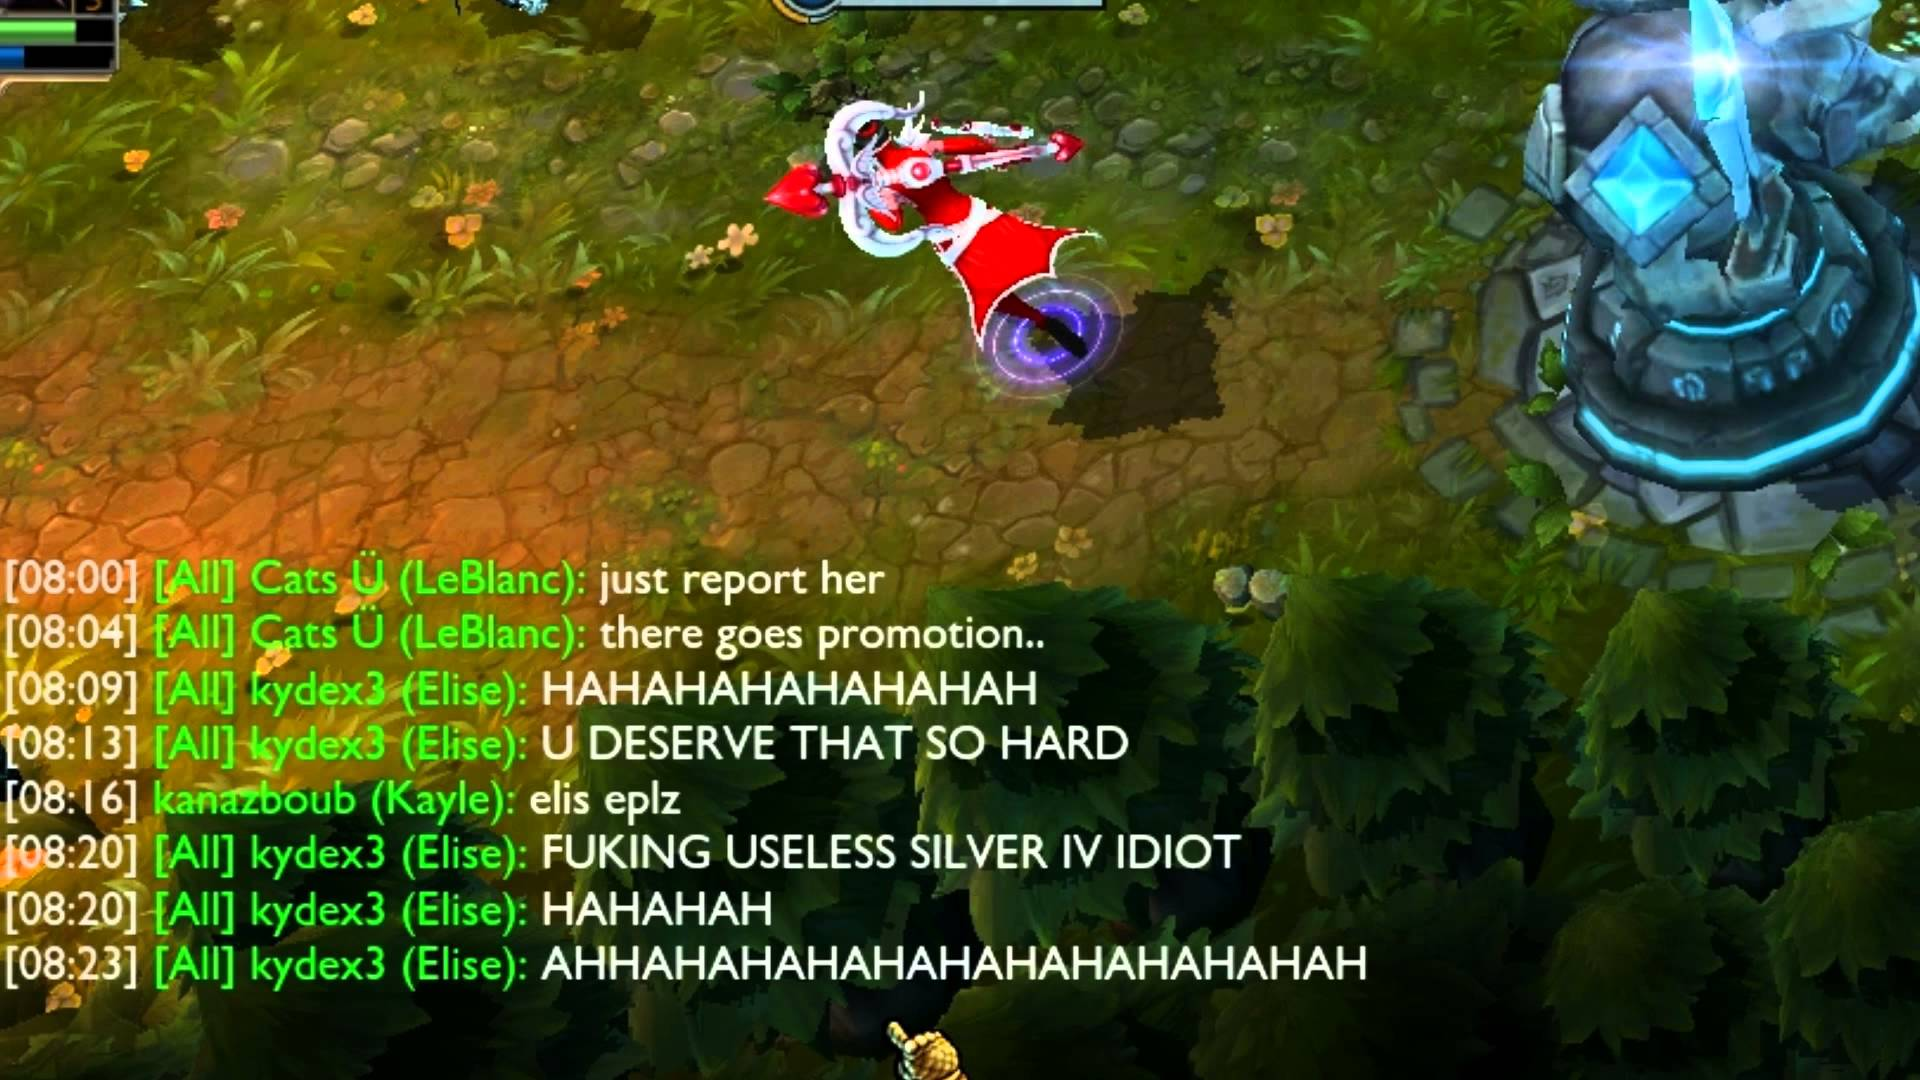
\includegraphics[width=0.45\textwidth]{images/estadodelarte/ai/lol-toxic-capture}
	\centering
	\caption{Ejemplo de comportamiento tóxico en \citegame{league_of_legends}.}
	\label{lol-toxic-capture}
\end{figure}
